\documentclass[a4paper,12pt]{article}
\usepackage{amssymb}
\usepackage{amsmath}
\usepackage[utf8]{inputenc} % Umlaute
\usepackage[ngerman]{babel} % Umlaute
\usepackage[T1]{fontenc}    % Umlaute
\usepackage[margin=2.5cm]{geometry}
\usepackage{booktabs}
\usepackage{lmodern}
\usepackage{titlesec}
\usepackage{longtable}
\usepackage{tabularx} % table
\usepackage{array}	%% ??
\usepackage[table]{xcolor}% http://ctan.org/pkg/xcolor
% Notwendig für Links im Text
\usepackage{hyperref}
%%\usepackage{svg}
% glossar, see http://en.wikibooks.org/wiki/LaTeX/Glossary
% muss NACH hyperref geladen werden, sonst funktionieren die Links nicht
\usepackage[toc]{glossaries}

% Kompatibilität
\ifx\pdftexversion\undefined
\usepackage[dvips]{graphicx}
\else
\usepackage[pdftex]{graphicx}
\DeclareGraphicsRule{*}{mps}{*}{}
\fi
\setlength{\parindent}{0pt}

%valle will Automaten verwenden
\usepackage{tikz}
\usetikzlibrary{automata, positioning, arrows}

%irgendwas mit section formatierung (titlesec package)
\titleformat{\paragraph}[hang]{\normalfont\normalsize\bfseries}{\theparagraph}{1em}{}
%%%%%%%%%%%%%%%%%%%%%%%%%%%%%%%%%%%%%%%%%%%%%%%%%%%%%%%%%%%%%%%%%%%%%%
% Variablen                                 						 %
%%%%%%%%%%%%%%%%%%%%%%%%%%%%%%%%%%%%%%%%%%%%%%%%%%%%%%%%%%%%%%%%%%%%%%
\newcommand{\authorName}{Tec O'Brain (Entwickler: David Höglinger, Jan Ettrich, Erwin Müller, Benedikt Rittner, Valentin Quapil)}
\newcommand{\auftraggeber}{Karlsruhe Institute of Technology (Teco)}
\newcommand{\auftragnehmer}{\authorName}
\newcommand{\projektName}{Implementierung Earables}
\newcommand{\tags}{\authorName, Architektur, Implementierung, KIT, Informatik, PSE}
\newcommand{\documentVersion}{1.0}
\title{\projektName}
\date{\today}
\author{Tec O'Brain}

%%%%%%%%%%%%%%%%%%%%%%%%%%%%%%%%%%%%%%%%%%%%%%%%%%%%%%%%%%%%%%%%%%%%%%
% PDF Meta information                                 				 %
%%%%%%%%%%%%%%%%%%%%%%%%%%%%%%%%%%%%%%%%%%%%%%%%%%%%%%%%%%%%%%%%%%%%%%
\hypersetup{
  pdfauthor   = {\authorName},
  pdfkeywords = {\tags},
  pdftitle    = {\projektName)}
}

%%%%%%%%%%%%%%%%%%%%%%%%%%%%%%%%%%%%%%%%%%%%%%%%%%%%%%%%%%%%%%%%%%%%%%
% Create a shorter version for tables. DO NOT CHANGE               	 %
%%%%%%%%%%%%%%%%%%%%%%%%%%%%%%%%%%%%%%%%%%%%%%%%%%%%%%%%%%%%%%%%%%%%%%
\newcommand\addrow[2]{#1 &#2\\ }

\newcommand\addheading[2]{#1 &#2\\ \hline}
\newcommand\tabularhead{\begin{tabular}{lp{13cm}}
\hline
}

\newcommand\addmulrow[2]{ \begin{minipage}[t][][t]{2.5cm}#1\end{minipage}%
   &\begin{minipage}[t][][t]{8cm}
    \begin{enumerate} #2   \end{enumerate}
    \end{minipage}\\ }

\newenvironment{usecase}{\tabularhead}
{\hline\end{tabular}}

\usepackage{microtype}
%%%%%%%%%%%%%%%%%%%%%%%%%%%%%%%%%%%%%%%%%%%%%%%%%%%%%%%%%%%%%%%%%%%%%%
% GLOSSARY ENTRIES                 	                              	 %
%%%%%%%%%%%%%%%%%%%%%%%%%%%%%%%%%%%%%%%%%%%%%%%%%%%%%%%%%%%%%%%%%%%%%%


%%%%%%%%%%%%%%%%%%%%%%%%%%%%%%%%%%%%%%%%%%%%%%%%%%%%%%%%%%%%%%%%%%%%%%
% THE DOCUMENT BEGINS             	                              	 %
%%%%%%%%%%%%%%%%%%%%%%%%%%%%%%%%%%%%%%%%%%%%%%%%%%%%%%%%%%%%%%%%%%%%%%
\begin{document}
\pagenumbering{roman}
\begin{titlepage}
\maketitle
\thispagestyle{empty} % no page number

\begin{verbatim}












\end{verbatim}


  \begin{tabular}[t]{p{4 cm}p{8 cm}}
	Projekt:       & \projektName \\[1.2ex]
	Auftraggeber:  & \auftraggeber\\[1.2ex]
	Auftragnehmer: & \auftragnehmer\\[1.2ex]
  \end{tabular}


\begin{tabular}[t]{|p{4 cm}|p{8 cm}|}
\hline
\textbf{Datum} & \textbf{Autor(en)} \\
\hline
\hline
\today & \authorName \\
\hline
\end{tabular}
\end{titlepage}
         % Deckblatt.tex laden und einfügen
\setcounter{page}{2}
\tableofcontents          % Inhaltsverzeichnis ausgeben
\clearpage
\pagenumbering{arabic}
%%%%%%%%%%%%%%%%%%%%%%%%%%%%%%%%%%%%%%% CONTENT %%%%%%%%%%%%%%%%%%%%%%%%%%%%%%%%%%%%%%%%%%%%%%%

\section{Einleitung}
Das nachfolgende Dokument spiegelt den Ablauf unserer Implementierungsphase wieder. Festgehalten wurden hauptsächlich Probleme, auf die wir beim Implementieren gestoßen sind, wie wir diese gelöst haben und welche Änderungen wir dafür am Entwurf vornehmen mussten. Zusätzlich wird die Implementierung der Erkennungsalgorithmen beschrieben. Eine visuelle Übersicht der einzelnen Aufgaben, die bei der Implementierung entstanden sind, werden durch das beigefügte Gantt Chart repräsentiert.\\
Insgesamt ist es uns durch durch unsere Teamarbeit gelungen, alle Muss- und Wunsch-Kriterien umzusetzen. Wir haben es geschafft, die Bibliothek, die für die Steuerung der Earables zuständig ist, als NuGet zu veröffentlichen. Bei den Änderungen, die wir am ursprünglichen Entwurf vornehme mussten, handelt es sich zum größten Teil um Kleinigkeiten.\\
Unser Workflow fand mit GitHub oder auch GitKraken statt. Jeder entwickelte auf seinem Branch seine Features und machte durch ein Pull-Request kenntlich, falls seine Feature fertig war. Issues wurden hauptsächlich auf dem Papier, aber auch mündlich festgehalten. Zur Überprüfung des Codes verwendeten wir Azure Pipelines.

\section{Implemetierung der Erkennungsalgorithmen}
\label{algorithmen}
Im Folgenden werden die implementierten Algorithmen für die Lauf-, Schritt-, PushUp- und  Sit-Up-Erkennung erläutert. Die konkreten Variablen und Benennungen sind im Code entsprechend auffindbar und ausführlich kommentiert.
\subsection{Warum Threshold-Algorithmen?}
Wir haben uns bewusst dafür entschieden, auf maschinelles Lernen im Sinne von Neuronalen Netzen zu verzichten und stattdessen einen heuristischen Ansatz zu wählen.\\
 Bei einem Threshold-Ansatz bestehen wesentliche Teile der Entscheidung darin, ob ein bestimmter Schwellenwert von einem Messwert überschritten wird.
\paragraph{Vorteile}
Dies hat einerseits den Grund, dass wir selbst wenig Erfahrung mit neuronalen Netzen haben. Andererseits wollten wir den Fokus in unserer App weniger auf Perfektion legen, und mehr darauf, Anwendungsszenarien von Bewegungserkennung mit Kopfhöhrern zu modellieren: Die App ist auch ein Experiment, um herauszufinden, was man vielleicht mit Earables besser erkennen kann als mit einem Fitness-Armband. Bei der Implementierung hat sich herausgestellt, dass für unsere Zwecke ein Threshold-Algorithmus ausreichend ist. Man lernt bei der Entwicklung auch selbst sehr gut, in wie weit man mit den Sensoren bestimmte Bewegungen erkennen kann. Dieses Grundverständnis zu erreichen ist für uns wichtiger als ein perfekt funktionierender Algorithmus.\\
Zusätzlich muss man sagen, dass jeder Algorithmus durch die Service-Struktur der Activities leicht ausgetauscht werden kann.
\paragraph{Nachteile}
Ein Ansatz mit maschinellem Lernen bzw. ein vor dem release trainiertes neuronales Netz würde vermutlich akkuratere Ergebnisse liefern. 
\subsection{Benennung der Messwerte}
Die Kopfhöhrer befinden sich nicht immer exakt in dieser Position, sondern können zu den Sensorachsen leicht verdeht sein. Wir bezeichnen (aus der Perspektive des/der Tragenden) die (Mess-)Werte:
\begin{itemize}
	\item Beschleunigung nach unten in G: $AccX$
	\item Beschleunigung nach vorne in G: $AccY$
	\item Beschleunigung nach links in G: $AccZ$
	\item absolute Beschleunigung: $AccAbs = \sqrt{AccX^2+AccY^2+AccZ^2}$
	\item Drehbeschleunigung vorne-nach-rechts in Grad pro Sekunde: $GyroX$ 
	\item Drehbeschleunigung oben-nach-links in Grad pro Sekunde: $GyroY$ 
	\item Drehbeschleunigung oben-nach-vorne in Grad pro Sekunde: $GyroZ$ 
	\item absolute Drehbeschleunigung: $GyroAbs = \sqrt{GyroX^2+GyroY^2+GyroZ^2}$
	\item Samplingrate (Anzahl Messwerte pro Sekunde) in Hz: $freq$
\end{itemize}
Das sind alle für die Algorithmen verwendete Werte. Optional wird als Index der Zeitpunkt $i$ des Messwerts verwendet, wobei $i$ und $i+1$ aufeinanderfolgende Werte sind.
\subsection{Schritterkennung (StepActivityThreshold)}
\subsubsection{naiver Threshold-Ansatz}
Die Schritterkennung basiert auf einem klassischen Threshold-Ansatz:\\
erkenne Schritt, falls 
\begin{equation}
	AccAbs > 1.15
\end{equation}
Bei jedem Messwert wird die absolute Beschleunigung gemessen. Überschreitet sie einen bestimmten Schwellenwert (z.B. die 1.15-fache Erdbeschleunigung), wird ein Schritt erkannt.\\ 
Damit ein Schritt nicht mehrfach erkannt wird, erfolgt nach jedem Schritt eine Cooldown-Phase (z.B. 0.3 Sekunden lang), in der keine neuen Schritte mehr erkannt werden.
\paragraph{Erkenntnisse}
Schritte beim normalen Gehen werden immer erkannt, und zwar durch die Erschütterung (Beschleunigung nach unten) beim Auftreten. 
\begin{figure}
	\centering
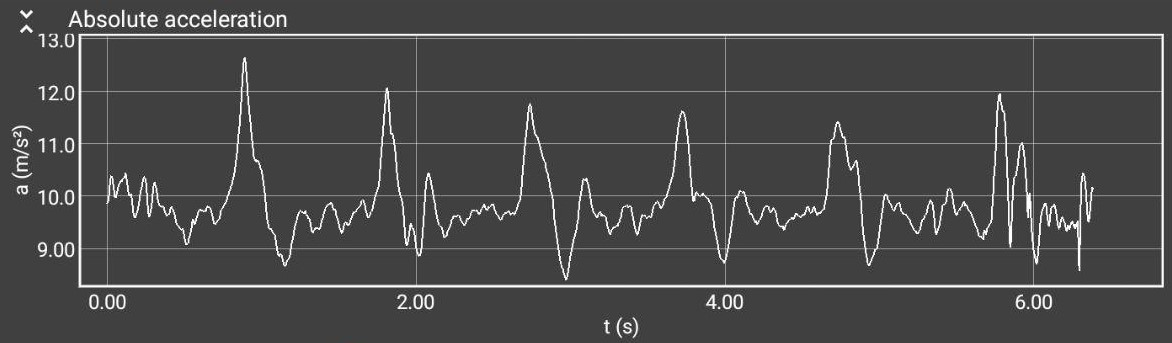
\includegraphics[width = 14cm]{bilder/steps.jpg}
	\caption{Absolute Beschleunigung beim Laufen, gemessen mit phyphox-App und Beschleunigungssensoren des Handys  (Beachte, dass $9,81 m/s^2 \approx 1 G$)).}
\end{figure} 
Allerdings werden auch viele andere Bewegungen (z.B. Kopfschütteln) erkannt.
\subsubsection{Verbesserter Ansatz}
Um die Anzahl der ``false positives'' zu verringern, wird jetzt eine zusätzliche Bedingung eingeführt:\\
Bei Schritten ist die Beschleunigung immer nach unten gerichtet. Daher wird jetzt zusätzlich gemessen, wo gerade vermutlich unten ist, indem ein Durchschnitt laufend aktualisiert wird. Ein sehr einfacher Ansatz ist dabei, den Durchschnitt exponentiell anzugleichen:
\begin{equation}
	avgAccX_i = (avgAccX_{i-1} * weight + AccX_i) /(weight + 1)
\end{equation}
Analog wird diese Berechnung auch für die anderen Koordinaten durchgeführt. Somit ergibt sich direkt ein \textbf{Vektor $AvgAcc$ der durchschnittlichen Beschleunigung, der als ``nach unten zeigend'' interpretiert werden kann}, da die Richtung der durchschnittlichen Beschleunigung mit der Richtung ``unten'' korreliert. Initialisiert werden die Werte, als ob sich die Earables in Ausgangsposition befinden (Kopf gerade). Wir haben hierbei die Gewichtung $weight$ von der Samplingrate abhängig gemacht, sodass geringerer Samplerate die Angleichung nicht deutlich langsamer erfolgt:
\begin{equation}
	weight = freq * 2
\end{equation}
Vergleicht man nun (in der visuellen Vorstellung des Verfahrens) den Vektor $AvgAcc$ mit dem Vektor, der die \textbf{aktuelle Beschleunigung $Acc$} repräsentiert, kann man den \textbf{Winkel $\alpha$} für die Klassifikation nutzen.\\
Im Algorithmus kann dabei der Cosinus des Winkels zwischen approximierter Standardbeschleunigung und aktueller Beschleunigung folgendermaßen berechnet werden:
\begin{equation}
	cos(\alpha) = \frac{avgAccX * AccX + avgAccY * AccY + avgAccZ * AccZ}{ AccAbs * AvgAccAbs },
\end{equation}
wobei $AvgAccAbs = \sqrt{avgAccX^2+avgAccY^2+avgAccZ^2}$ ist.\\
\newline
\noindent
\begin{minipage}{0.5\textwidth}
	Der Winkel wird in unserem Fall akzeptiert, falls $cos(\alpha) > 0.89$, also darf der Winkel um maximal 27 Grad abweichen. Die intuitive Erklärung für diese Klassifikation ist, dass eine Erschütterung beim Auftreten in etwa ``nach unten'' gerichtet ist, ansonsten muss es sich um eine andere Bewegung handeln.\\ 
	Diese Klassifikation hat sich als Erfahrungswert geeignet.
	Zusätzlich kann auch das Threshold jetzt relativ zur durchschnittlichen Beschleunigung berechnet werden:
	\begin{equation}
		AccAbs > 1.15 * AvgAccAbs
	\end{equation}
	
	So kann eine falsche Kalibrierung der Sensoren ausgeglichen werden.
\end{minipage}
\hspace{0.1\textwidth}
\begin{minipage}{0.35\textwidth}
	
%%erstellt mit https://www.mathcha.io/editor

\tikzset{every picture/.style={line width=0.75pt}} %set default line width to 0.75pt        

\begin{tikzpicture}[x=0.75pt,y=0.75pt,yscale=-1,xscale=1]
%uncomment if require: \path (0,410.90625); %set diagram left start at 0, and has height of 410.90625

%Shape: Arc [id:dp6141700786507858] 
\draw  [draw opacity=0][fill={rgb, 255:red, 81; green, 226; blue, 74 }  ,fill opacity=0.55 ] (374.18,293.16) .. controls (359.81,304.36) and (341.22,311.06) .. (320.96,310.93) .. controls (300.8,310.81) and (282.38,303.95) .. (268.17,292.67) -- (321.44,234.95) -- cycle ; \draw  [color={rgb, 255:red, 226; green, 74; blue, 79 }  ,draw opacity=0 ] (374.18,293.16) .. controls (359.81,304.36) and (341.22,311.06) .. (320.96,310.93) .. controls (300.8,310.81) and (282.38,303.95) .. (268.17,292.67) ;
%Straight Lines [id:da39478853698383154] 
\draw [color={rgb, 255:red, 74; green, 144; blue, 226 }  ,draw opacity=1 ]   (321.5,235) -- (321,308.36) ;
\draw [shift={(320.97,311.36)}, rotate = 270.39] [fill={rgb, 255:red, 74; green, 144; blue, 226 }  ,fill opacity=1 ][line width=0.08]  [draw opacity=0] (8.93,-4.29) -- (0,0) -- (8.93,4.29) -- cycle    ;
\draw [shift={(321.5,235)}, rotate = 90.39] [color={rgb, 255:red, 74; green, 144; blue, 226 }  ,draw opacity=1 ][fill={rgb, 255:red, 74; green, 144; blue, 226 }  ,fill opacity=1 ][line width=0.75]      (0, 0) circle [x radius= 3.35, y radius= 3.35]   ;
%Shape: Arc [id:dp5049979934092728] 
\draw  [draw opacity=0][fill={rgb, 255:red, 226; green, 74; blue, 77 }  ,fill opacity=0.29 ] (268.17,292.67) .. controls (250.51,278.62) and (239.38,257.74) .. (239.52,234.48) .. controls (239.79,192.52) and (276.7,158.73) .. (321.98,159.02) .. controls (367.25,159.3) and (403.74,193.55) .. (403.48,235.52) .. controls (403.33,258.91) and (391.79,279.76) .. (373.77,293.59) -- (321.5,235) -- cycle ; \draw  [color={rgb, 255:red, 226; green, 74; blue, 79 }  ,draw opacity=0 ] (268.17,292.67) .. controls (250.51,278.62) and (239.38,257.74) .. (239.52,234.48) .. controls (239.79,192.52) and (276.7,158.73) .. (321.98,159.02) .. controls (367.25,159.3) and (403.74,193.55) .. (403.48,235.52) .. controls (403.33,258.91) and (391.79,279.76) .. (373.77,293.59) ;
%Shape: Arc [id:dp7716732689668444] 
\draw  [draw opacity=0][fill={rgb, 255:red, 74; green, 144; blue, 226 }  ,fill opacity=0.22 ] (322.06,247) .. controls (321.85,247) and (321.64,247) .. (321.42,247) .. controls (317.86,246.98) and (314.51,246.38) .. (311.63,245.35) -- (321.5,235) -- cycle ; \draw  [color={rgb, 255:red, 74; green, 144; blue, 226 }  ,draw opacity=1 ] (322.06,247) .. controls (321.85,247) and (321.64,247) .. (321.42,247) .. controls (317.86,246.98) and (314.51,246.38) .. (311.63,245.35) ;
%Straight Lines [id:da07556207680782712] 
\draw [color={rgb, 255:red, 74; green, 144; blue, 226 }  ,draw opacity=1 ]   (321.5,235) -- (360.52,348.48) ;
\draw [shift={(361.5,351.32)}, rotate = 251.01999999999998] [fill={rgb, 255:red, 74; green, 144; blue, 226 }  ,fill opacity=1 ][line width=0.08]  [draw opacity=0] (8.93,-4.29) -- (0,0) -- (8.93,4.29) -- cycle    ;
\draw [shift={(321.5,235)}, rotate = 71.02] [color={rgb, 255:red, 74; green, 144; blue, 226 }  ,draw opacity=1 ][fill={rgb, 255:red, 74; green, 144; blue, 226 }  ,fill opacity=1 ][line width=0.75]      (0, 0) circle [x radius= 3.35, y radius= 3.35]   ;
%Shape: Arc [id:dp542059610762009] 
\draw  [draw opacity=0][fill={rgb, 255:red, 74; green, 144; blue, 226 }  ,fill opacity=0.22 ] (334.22,272.18) .. controls (330.14,272.86) and (325.88,273.21) .. (321.49,273.18) .. controls (321.41,273.18) and (321.32,273.18) .. (321.24,273.18) -- (321.73,235.77) -- cycle ; \draw  [color={rgb, 255:red, 74; green, 144; blue, 226 }  ,draw opacity=1 ] (334.22,272.18) .. controls (330.14,272.86) and (325.88,273.21) .. (321.49,273.18) .. controls (321.41,273.18) and (321.32,273.18) .. (321.24,273.18) ;

% Text Node
\draw (300,315) node  [font=\footnotesize,color={rgb, 255:red, 74; green, 144; blue, 226 }  ,opacity=1 ]  {$AvgAcc$};
% Text Node
\draw (309,256) node  [font=\footnotesize,color={rgb, 255:red, 74; green, 144; blue, 226 }  ,opacity=1 ]  {$37^{\circ}$};
% Text Node
\draw (366,325) node  [font=\footnotesize,color={rgb, 255:red, 74; green, 144; blue, 226 }  ,opacity=1 ]  {$Acc$};
% Text Node
\draw (328,264) node  [font=\footnotesize,color={rgb, 255:red, 74; green, 144; blue, 226 }  ,opacity=1 ,rotate=-349.43]  {$\alpha $};


\end{tikzpicture}\\

	Visualisierung: als Schritt akzeptierte Beschleunigung $Acc$
\end{minipage}
\vspace{0.5cm}\\

Da alle Vergleiche relativ erfolgen, kann zur Schritterkennung der Sensor auch falsch orientiert sein. Die Erkennung funktioniert trotzdem korrekt, da sie sich an die relative Richtung der Erdbeschleunigung anpasst.\\
\paragraph{Ausprobieren}
Die folgende Version der App unter Menüpunkt Debug ist zum Ausprobieren geeignet (Algorithmus hier im DebugViewModel, andere Thresholds / Strategien können einfach ausprobiert werden): 
\href{https://github.com/vlle1/earablesKIT/tree/b8b34bbe0716ddb37c5afbd315e91d7f11c0270d}{earablesKIT/debugView/Schritterkennung\_Version\_3}\\
Dabei werden auch einige Debug-Informationen auf dem Display angezeigt, z.B. der erkannte Winkel.

\subsection{Lauferkennung (RunningActivityThreshold)}
Dieser Algorithmus ist sehr simpel und basiert auf dem Schritterkennungsalgorithmus: 
\newline

% erstellt mit https://www.mathcha.io/editor

\tikzset{every picture/.style={line width=0.75pt}} %set default line width to 0.75pt        
\begin{center}
\begin{tikzpicture}[x=0.75pt,y=0.75pt,yscale=-1,xscale=1]
%uncomment if require: \path (0,410.90625); %set diagram left start at 0, and has height of 410.90625

%Shape: Circle [id:dp6318133684241805] 
\draw   (137,259) .. controls (137,245.19) and (148.19,234) .. (162,234) .. controls (175.81,234) and (187,245.19) .. (187,259) .. controls (187,272.81) and (175.81,284) .. (162,284) .. controls (148.19,284) and (137,272.81) .. (137,259) -- cycle ;
%Straight Lines [id:da6926894193378876] 
\draw    (87.5,259) -- (134,259) ;
\draw [shift={(137,259)}, rotate = 180] [fill={rgb, 255:red, 0; green, 0; blue, 0 }  ][line width=0.08]  [draw opacity=0] (8.93,-4.29) -- (0,0) -- (8.93,4.29) -- cycle    ;
\draw [shift={(87.5,259)}, rotate = 0] [color={rgb, 255:red, 0; green, 0; blue, 0 }  ][fill={rgb, 255:red, 0; green, 0; blue, 0 }  ][line width=0.75]      (0, 0) circle [x radius= 3.35, y radius= 3.35]   ;
%Shape: Circle [id:dp0026005274455069838] 
\draw   (214,323) .. controls (214,309.19) and (225.19,298) .. (239,298) .. controls (252.81,298) and (264,309.19) .. (264,323) .. controls (264,336.81) and (252.81,348) .. (239,348) .. controls (225.19,348) and (214,336.81) .. (214,323) -- cycle ;
%Curve Lines [id:da24747493565188639] 
\draw    (187,259) .. controls (213.54,258.07) and (235.88,268.28) .. (238.76,295.02) ;
\draw [shift={(239,298)}, rotate = 267.04] [fill={rgb, 255:red, 0; green, 0; blue, 0 }  ][line width=0.08]  [draw opacity=0] (8.93,-4.29) -- (0,0) -- (8.93,4.29) -- cycle    ;

%Curve Lines [id:da49971886799260323] 
\draw    (214,323) .. controls (185.38,327.88) and (166.65,316.74) .. (162.36,286.83) ;
\draw [shift={(162,284)}, rotate = 443.77] [fill={rgb, 255:red, 0; green, 0; blue, 0 }  ][line width=0.08]  [draw opacity=0] (8.93,-4.29) -- (0,0) -- (8.93,4.29) -- cycle    ;


% Text Node
\draw (239,323) node   [align=left] {laufe};
% Text Node
\draw (162,259) node   [align=left] {stehe};
% Text Node
\draw (246,263.04) node  [font=\normalsize] [align=left] {Schritt wird\\ \ \ \ \ \ \ \ erkannt};
% Text Node
\draw (125,320.04) node  [font=\normalsize] [align=left] {1 Sekunde lang \\keinen Schritt erkannt};


\end{tikzpicture}
\end{center}

Da der Nutzer seine Schrittfrequenz oft unregelmäßig ändert, macht es wenig Sinn, das Timeout (hier eine Sekunde) daran relativ anzupassen.\\
Bei sehr zuverlässiger Schritterkennung könnte man das Timeout allerdings verringern; aktuell soll aber vor allem ``laufe'' nicht unterbrochen werden, falls z.B. ein einzelner Schritt nicht erkannt wurde.\\ 

\subsection{Liegestützen-Erkennung (PushUpActivityThreshold)}
Hier wird ein Zustandsautomat mit vier Zuständen verwendet (die Cooldowns sind eigentlich keine eigenen Zustände, aber so ist es besser visualisiert). 
\paragraph{Grundlagen}
Im Wesentlichen basiert der Algorithmus auf dem Fakt, dass die absolute Beschleunigung der Sensoren nur dann geringer als 1G sein kann, wenn die Kopfhöhrer sich Richtung Boden beschleunigen.\\
Es wurde mit Cooldowns gearbeitet, um zu vermeiden, dass durch kurze Bewegungen fälschlicherweise Liegestütze gezählt werden.\\
Außerdem sollte der Algorithmus unempflindlich sein, wenn der Nutzer (etwa aus Erschöpfung oder Verzweiflung an der Text-to-Speech-Stimme im ListenAndPerform Modus) seinen Kopf zur Seite dreht, hängen lässt oder Ähnliches. Dies wird dadurch erreicht, dass nur die absolute Beschleunigung berücksichtigt wird.
\paragraph{Wertverlauf}
Bei einer einzelnen Liegestütze ergibt sich der folgende Verlauf für die absolute Beschleunigung.\\
\begin{figure}[ht]
	\centering
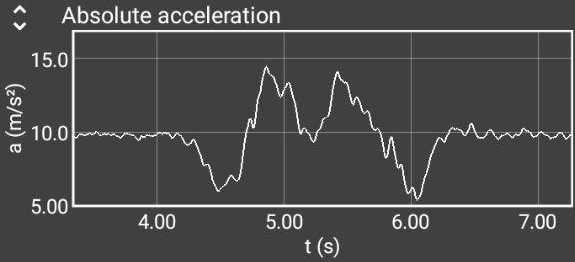
\includegraphics[width = 10cm]{bilder/pushup_sample.jpg}
	\caption{Absolute Beschleunigung bei einer Liegestütze, gemessen mit phyphox-App und Beschleunigungssensoren des Handys (Beachte, dass $9,81 m/s^2 \approx 1 G$).}
\end{figure} 
Man kann sich bewusst machen, dass die absolute Beschleunigung der Kopfhöhrer in etwa proportional zum Druck ist, den man mit den Händen auf den Boden ausübt. So wird auch klar, wie die beiden Maxima im Verlauf zustande kommen: Erst bremst man die Abwärtsbewegung aus, dann drückt man sich wieder vom Boden weg. Analog gilt das auch für die beiden Minima. 
\paragraph{Zustandsautomat}
% erstellt mit https://www.mathcha.io/editor

\begin{center}
    



    \tikzset{every picture/.style={line width=0.75pt}} %set default line width to 0.75pt        

    \begin{tikzpicture}[x=0.75pt,y=0.75pt,yscale=-1,xscale=1]
    %uncomment if require: \path (0,612.0170516967773); %set diagram left start at 0, and has height of 612.0170516967773
    
    %Shape: Circle [id:dp4115012649218517] 
    \draw   (172,454) .. controls (172,440.19) and (183.19,429) .. (197,429) .. controls (210.81,429) and (222,440.19) .. (222,454) .. controls (222,467.81) and (210.81,479) .. (197,479) .. controls (183.19,479) and (172,467.81) .. (172,454) -- cycle ;
    %Straight Lines [id:da06931047169438798] 
    \draw    (115.83,411.33) -- (173.11,438.06) ;
    \draw [shift={(175.83,439.33)}, rotate = 205.02] [fill={rgb, 255:red, 0; green, 0; blue, 0 }  ][line width=0.08]  [draw opacity=0] (8.93,-4.29) -- (0,0) -- (8.93,4.29) -- cycle    ;
    \draw [shift={(115.83,411.33)}, rotate = 25.02] [color={rgb, 255:red, 0; green, 0; blue, 0 }  ][fill={rgb, 255:red, 0; green, 0; blue, 0 }  ][line width=0.75]      (0, 0) circle [x radius= 3.35, y radius= 3.35]   ;
    %Shape: Circle [id:dp48735130026263906] 
    \draw   (87.97,510.93) .. controls (87.97,497.12) and (99.17,485.93) .. (112.97,485.93) .. controls (126.78,485.93) and (137.97,497.12) .. (137.97,510.93) .. controls (137.97,524.74) and (126.78,535.93) .. (112.97,535.93) .. controls (99.17,535.93) and (87.97,524.74) .. (87.97,510.93) -- cycle ;
    %Curve Lines [id:da6609208305880534] 
    \draw    (172,454) .. controls (144.45,455.9) and (121.39,465.86) .. (114.01,483.14) ;
    \draw [shift={(112.97,485.93)}, rotate = 287.53] [fill={rgb, 255:red, 0; green, 0; blue, 0 }  ][line width=0.08]  [draw opacity=0] (8.93,-4.29) -- (0,0) -- (8.93,4.29) -- cycle    ;
    
    %Shape: Circle [id:dp9177005648524454] 
    \draw   (172,561) .. controls (172,547.19) and (183.19,536) .. (197,536) .. controls (210.81,536) and (222,547.19) .. (222,561) .. controls (222,574.81) and (210.81,586) .. (197,586) .. controls (183.19,586) and (172,574.81) .. (172,561) -- cycle ;
    %Curve Lines [id:da8997751532087288] 
    \draw    (112.97,535.93) .. controls (116.81,554.2) and (143.04,558.63) .. (169.16,560.77) ;
    \draw [shift={(172,561)}, rotate = 184.38] [fill={rgb, 255:red, 0; green, 0; blue, 0 }  ][line width=0.08]  [draw opacity=0] (8.93,-4.29) -- (0,0) -- (8.93,4.29) -- cycle    ;
    
    %Shape: Circle [id:dp5913276051851417] 
    \draw   (317,564) .. controls (317,550.19) and (328.19,539) .. (342,539) .. controls (355.81,539) and (367,550.19) .. (367,564) .. controls (367,577.81) and (355.81,589) .. (342,589) .. controls (328.19,589) and (317,577.81) .. (317,564) -- cycle ;
    %Curve Lines [id:da588437346756167] 
    \draw    (222,561) .. controls (237.42,560.93) and (286.38,561.86) .. (314.07,563.79) ;
    \draw [shift={(317,564)}, rotate = 184.38] [fill={rgb, 255:red, 0; green, 0; blue, 0 }  ][line width=0.08]  [draw opacity=0] (8.93,-4.29) -- (0,0) -- (8.93,4.29) -- cycle    ;
    
    %Shape: Circle [id:dp9891196847216435] 
    \draw   (376.97,517.93) .. controls (376.97,504.12) and (388.17,492.93) .. (401.97,492.93) .. controls (415.78,492.93) and (426.97,504.12) .. (426.97,517.93) .. controls (426.97,531.74) and (415.78,542.93) .. (401.97,542.93) .. controls (388.17,542.93) and (376.97,531.74) .. (376.97,517.93) -- cycle ;
    %Curve Lines [id:da6447447682801046] 
    \draw    (367,564) .. controls (386.74,567.76) and (401.16,560.86) .. (401.98,545.89) ;
    \draw [shift={(401.97,542.93)}, rotate = 446.63] [fill={rgb, 255:red, 0; green, 0; blue, 0 }  ][line width=0.08]  [draw opacity=0] (8.93,-4.29) -- (0,0) -- (8.93,4.29) -- cycle    ;
    
    %Curve Lines [id:da7537207989164001] 
    \draw    (314.83,453.33) .. controls (305.94,441.05) and (251.26,440.36) .. (223.34,445.81) ;
    \draw [shift={(220.83,446.33)}, rotate = 347.47] [fill={rgb, 255:red, 0; green, 0; blue, 0 }  ][line width=0.08]  [draw opacity=0] (8.93,-4.29) -- (0,0) -- (8.93,4.29) -- cycle    ;
    
    %Shape: Circle [id:dp7322215580168285] 
    \draw   (311.97,466.93) .. controls (311.97,453.12) and (323.17,441.93) .. (336.97,441.93) .. controls (350.78,441.93) and (361.97,453.12) .. (361.97,466.93) .. controls (361.97,480.74) and (350.78,491.93) .. (336.97,491.93) .. controls (323.17,491.93) and (311.97,480.74) .. (311.97,466.93) -- cycle ;
    %Curve Lines [id:da44315821397943034] 
    \draw    (393.97,494.93) .. controls (390.04,483.91) and (381.72,471.63) .. (364.73,467.51) ;
    \draw [shift={(361.97,466.93)}, rotate = 370.22] [fill={rgb, 255:red, 0; green, 0; blue, 0 }  ][line width=0.08]  [draw opacity=0] (8.93,-4.29) -- (0,0) -- (8.93,4.29) -- cycle    ;
    
    
    % Text Node
    \draw (197,454) node   [align=left] {oben};
    % Text Node
    \draw (83,457.04) node  [font=\normalsize] [align=left] {AbsAcc < 0.8};
    % Text Node
    \draw (112.97,510.93) node   [align=left] {runter};
    % Text Node
    \draw (283,433.04) node  [font=\normalsize] [align=left] {AbsAcc < 0.8};
    % Text Node
    \draw (78,559.04) node  [font=\normalsize] [align=left] {AbsAcc > 1.15};
    % Text Node
    \draw (197,561) node   [align=left] {unten};
    % Text Node
    \draw (266,575.04) node  [font=\normalsize] [align=left] {nach 0.3 s};
    % Text Node
    \draw (342,564) node   [align=left] {unten'};
    % Text Node
    \draw (428,573.04) node  [font=\normalsize] [align=left] {AbsAcc > 1.15};
    % Text Node
    \draw (401.97,517.93) node   [align=left] {hoch};
    % Text Node
    \draw (336.97,466.93) node   [align=left] {hoch'};
    % Text Node
    \draw (411,461.04) node  [font=\normalsize] [align=left] {nach 0.3 s};
    
    
    \end{tikzpicture}
    
\end{center}

\paragraph{Weitere Beobachtungen}
Man könnte jetzt noch zusätzlich einen Timeout einführen (hält Zustand ``abwärts'' oder ``aufwärts'' zu lange, wurde die Liegestütze vermutlich abgebrochen) und die verschiedenen Thresholds feiner anpassen, um die Erkennung noch weiter zu verbessern.\\
Der Algorithmus kommt an seine Grenzen, wenn man die Liegestütze extrem schnell ausführt (der Cooldown könnte an die Intensität der Beschleunigung angepasst werden), oder extrem langsam ausführt (da dann die Thresholds nicht mehr überschritten werden). Außerdem wird ab und zu schon eine Liegestütze erkannt, während man noch (zum Beispiel aus dem Stand) in die Startposition geht. Um diese Probleme zu umgehen wäre eine grundlegend andere Datenaufbereitung notwendig, beispielsweise mit einem Kalman-Filter.\\
Der Algorithmus könnte übrigens auch äquivalent für Kniebeugen verwendet werden.
\paragraph{Ausprobieren}
Die folgende Version der App unter Menüpunkt Debug ist zum Ausprobieren geeignet (Algorithmus hier im DebugViewModel, andere Thresholds / Strategien können einfach ausprobiert werden): 
\href{https://github.com/vlle1/earablesKIT/commit/6a4999ac8e2613298a6e6dd9bc85092ddd1b6133}{earablesKIT/debugView/Liegestütze-Erkennung}\\
Dabei werden auch einige Debug-Informationen auf dem Display angezeigt, die am grüßten angezeigte Zahl entspricht hier dem Zustand des Automaten: 0 (oben), 1 (runter), 2 (unten) bzw. 3 (hoch).

\subsection{Situps-Erkennung (SitUpActivityThreshold)}
\paragraph{Voraussetzung} 
Im Gegensatz zu den anderen Algorithmen gehen wir bei Situps davon aus, dass die Benutzer ihren Kopf während der Übung immer nach vorne ausrichten. Das liegt daran, dass wir das Gyroskop zur Erkennung mitbenutzen wollten, was quasi unmöglich wird, wenn der Kopf seitlich verdreht ist.\\
Der Nutzer sollte außerdem die ``alten SitUps'' machen, d.h. er bewegt seinen Kopf bis in die aufrecht sitzende Position. Hier soll der Algorithmus darauf achten, dass ``halbe Situps'' (Crunches) nicht gewertet werden.
\paragraph{Algorithmus}
Es handelt sich wieder um einen Zustandsautomaten mit vier Zuständen.\\
Der Algorithmus nutzt hier sowohl Gyroskop als auch Accelerometer. Die Drehbewegung des Kopfes bei der Ausführung von Situps ist das stärkste Merkmal. So muss $GyroZ$ beim aufrichten einen hohen positiven Wert haben, bei der Abwärtsbewegung einen entsprechenden negativen Wert.\\
Um ähnliche Bewegungen (z.B. nicken) auszuschließen, wird zusätzlich die Beschleunigung nach vorne ($AccY$) betrachtet. Diese muss zu Start der Übung sehr hoch sein (allerdings negativ, da ja nach hinten), da der Nutzer mit dem Kopf nach oben schaut; wenn der Nutzer aufrecht sitzt, sollte sie kurze Zeit quasi null sein (da er aber währenddessen nach hinten beschleunigt ist sie tatsächlich kurz positiv).\\
Durch die Kombination dieser Merkmale der Bewegung benötigt die Klassifikation keinerlei Cooldown, da es (zumindest versehentlich oder wenn man den Algorithmus nicht kennt) unwahrscheinlich ist, einen vollen Zyklus nur durch Wackeln mit dem Kopf oder ähnliches in kürzerer Zeit zu durchlaufen.
\paragraph{Zustandsautomat}
% erstellt mit https://www.mathcha.io/editor

\begin{center}
    


\tikzset{every picture/.style={line width=0.75pt}} %set default line width to 0.75pt        

\begin{tikzpicture}[x=0.75pt,y=0.75pt,yscale=-1,xscale=1]
%uncomment if require: \path (0,612.0170516967773); %set diagram left start at 0, and has height of 612.0170516967773

%Shape: Circle [id:dp4115012649218517] 
\draw   (172,454) .. controls (172,440.19) and (183.19,429) .. (197,429) .. controls (210.81,429) and (222,440.19) .. (222,454) .. controls (222,467.81) and (210.81,479) .. (197,479) .. controls (183.19,479) and (172,467.81) .. (172,454) -- cycle ;
%Straight Lines [id:da06931047169438798] 
\draw    (120.83,570.67) -- (172.83,570.35) ;
\draw [shift={(175.83,570.33)}, rotate = 539.65] [fill={rgb, 255:red, 0; green, 0; blue, 0 }  ][line width=0.08]  [draw opacity=0] (8.93,-4.29) -- (0,0) -- (8.93,4.29) -- cycle    ;
\draw [shift={(120.83,570.67)}, rotate = 359.65] [color={rgb, 255:red, 0; green, 0; blue, 0 }  ][fill={rgb, 255:red, 0; green, 0; blue, 0 }  ][line width=0.75]      (0, 0) circle [x radius= 3.35, y radius= 3.35]   ;
%Shape: Circle [id:dp48735130026263906] 
\draw   (103.97,506.93) .. controls (103.97,493.12) and (115.17,481.93) .. (128.97,481.93) .. controls (142.78,481.93) and (153.97,493.12) .. (153.97,506.93) .. controls (153.97,520.74) and (142.78,531.93) .. (128.97,531.93) .. controls (115.17,531.93) and (103.97,520.74) .. (103.97,506.93) -- cycle ;
%Curve Lines [id:da6609208305880534] 
\draw    (172,454) .. controls (153.5,455.61) and (140.75,455.66) .. (130.12,479.27) ;
\draw [shift={(128.97,481.93)}, rotate = 292.46] [fill={rgb, 255:red, 0; green, 0; blue, 0 }  ][line width=0.08]  [draw opacity=0] (8.93,-4.29) -- (0,0) -- (8.93,4.29) -- cycle    ;

%Shape: Circle [id:dp9177005648524454] 
\draw   (172,561) .. controls (172,547.19) and (183.19,536) .. (197,536) .. controls (210.81,536) and (222,547.19) .. (222,561) .. controls (222,574.81) and (210.81,586) .. (197,586) .. controls (183.19,586) and (172,574.81) .. (172,561) -- cycle ;
%Curve Lines [id:da8997751532087288] 
\draw    (128.97,531.93) .. controls (132.81,550.2) and (144.14,558.35) .. (169.22,560.76) ;
\draw [shift={(172,561)}, rotate = 184.38] [fill={rgb, 255:red, 0; green, 0; blue, 0 }  ][line width=0.08]  [draw opacity=0] (8.93,-4.29) -- (0,0) -- (8.93,4.29) -- cycle    ;

%Shape: Circle [id:dp9891196847216435] 
\draw   (236.97,506.93) .. controls (236.97,493.12) and (248.17,481.93) .. (261.97,481.93) .. controls (275.78,481.93) and (286.97,493.12) .. (286.97,506.93) .. controls (286.97,520.74) and (275.78,531.93) .. (261.97,531.93) .. controls (248.17,531.93) and (236.97,520.74) .. (236.97,506.93) -- cycle ;
%Curve Lines [id:da6447447682801046] 
\draw    (222,561) .. controls (242.85,559.73) and (250.17,550.55) .. (260.49,534.28) ;
\draw [shift={(261.97,531.93)}, rotate = 482.14] [fill={rgb, 255:red, 0; green, 0; blue, 0 }  ][line width=0.08]  [draw opacity=0] (8.93,-4.29) -- (0,0) -- (8.93,4.29) -- cycle    ;

%Curve Lines [id:da44315821397943034] 
\draw    (253.97,483.93) .. controls (250.04,472.91) and (241.72,460.63) .. (224.73,456.51) ;
\draw [shift={(221.97,455.93)}, rotate = 370.22] [fill={rgb, 255:red, 0; green, 0; blue, 0 }  ][line width=0.08]  [draw opacity=0] (8.93,-4.29) -- (0,0) -- (8.93,4.29) -- cycle    ;


% Text Node
\draw (197,454) node   [align=left] {oben};
% Text Node
\draw (103,456.04) node  [font=\normalsize] [align=left] {AccY > 0};
% Text Node
\draw (128.97,506.93) node   [align=left] {runter};
% Text Node
\draw (197,561) node   [align=left] {unten};
% Text Node
\draw (290,459.04) node  [font=\normalsize] [align=left] {GyroZ > 100};
% Text Node
\draw (261.97,506.93) node   [align=left] {hoch};
% Text Node
\draw (280,562.04) node  [font=\normalsize] [align=left] {AccY< -1};
% Text Node
\draw (88,550.04) node  [font=\normalsize] [align=left] {GyroZ < -100};


\end{tikzpicture}

\end{center}
\paragraph{Beobachtungen}
Bei diesem Bewegungsablauf gibt es sehr wenige ``false positives'', d.h. die Bedingungen sind so speziefisch, dass kaum eine andere Bewegung als Situp erkannt werden sollte.\\
Oft bewegt man sich nicht ganz weit genug nach vorne, daher werden manche SitUps nich korrekt gezählt. Hier ist der Algorithmus also stark von der Auslegung der Übung abhängig (man könnte die Beschleunigungsbedingung im Zustand ``oben'' dann entsprechend weglassen).\\
Aus der Nutzerperspektive wäre ein Ton oder eine Anzeige sinnvoll, wenn Zustand ``oben'' erreicht wurde. Dies haben wir in unserem Entwurf allerdings nicht berücksichtigt und ist eher eine Idee, die erst am Ende der Implemetierung zustande kam.\\
Eine weitere Schwachstelle ist außerdem, dass die Kopfhöhrer im Ohr etwas verschieden gedreht werden können; sind sie hier zu arg verdreht, funktioniert der Algorithmus sofort nicht mehr, da die Richtung durch die Beschränkung auf $AccY$ vorgegeben ist.
\paragraph{Ausprobieren}
Die folgende Version der App unter Menüpunkt Debug ist zum Ausprobieren geeignet (Algorithmus hier im DebugViewModel, andere Thresholds / Strategien können einfach ausprobiert werden): 
\href{https://github.com/vlle1/earablesKIT/tree/cd774e370156ea3d13eff2879a2d7f0f7d541260}{earablesKIT/debugView/SitUps-Erkennung}\\
Dabei werden auch einige Debug-Informationen auf dem Display angezeigt, die am grüßten angezeigte Zahl entspricht hier dem Zustand des Automaten: 0 (unten), 1 (hoch), 2 (oben) bzw. 3 (runter).
\clearpage

\section{Probleme und Änderungen am Entwurf}
\label{aenderungen}
\paragraph{Legende}
Im Folgenden wird bei der Auflistung der Methodensignaturen und Attribute UML-Syntax verwendet.\\
Dabei bedeutet $-$ ``private'', $+$ ``public'' und \# ``protected''.
\subsection{Bibliothek}

\subsubsection{Umgang mit Exceptions}
\paragraph{Beschreibung}
Es war geplant, dass die meisten Schnittstellen der Bibliothek ein Boolean zurückgeben, der true ist, falls die Anweisung korrekt durchgeführt werden konnte und false , falls es Komplikationen gab.
Um besser auf Fehler und Exceptions zu reagieren macht es mehr Sinn, dass diese Methoden nichts zurückgeben und im Fehlerfall Exceptions schmeißen.\\
Dies wurde umgesetzt, falls sich der Nutzer mit der Schnittstelle IEarablesConnection mehrmals verbinden will, keine Verbindung aufgebaut werden konnte, eine ungültige SampleRate angegeben wurde (Werte zwischen 1 und 100 sind erlaubt) oder eine Aktion ausgeführt werden soll, die eine Verbindung voraussetzt, aber noch keine existiert.

\paragraph{Änderungen in Klasse IEarablesConnection}
Folgende Methoden haben nicht mehr den Rückgabetypen bool sondern void und schmeißen im Fehlerfall Exceptions:
\begin{itemize}
	\item[+] DisconnectFromDevice(): bool
	\item[+] StartSampling(): bool
	\item[+] StopSampling(): bool
\end{itemize} 
\paragraph{Hinzugefügte Exceptions}
Folgende Exception-Klassen mussten ergänzt werden:
\begin{itemize}
	\item[$-$] AllreadyConnectedException
	\item[$-$] ConnectionFailedException
	\item[$-$] InvalideSampleRateException
	\item[$-$] NoConnectionException
	\item[$-$] ChecksumException %man könnte noch überlegen die Rechtschreibfehler aus den AlreadyConnectedException und InvalidSampleRateException raus zu nehmen, müsste man dann aber auch konsequent im code so machen.
\end{itemize}
Die Exceptions werden geschmissen, falls bereits ein Gerät verbunden ist, keine Verbindung aufgebaut werden kann, der Wert der eingegebenen Samplerate nicht im richtigen Bereich (zwischen 1 und 100) liegt, die Checksumme nicht korrekt ist oder keine Verbindung vorhanden ist, diese aber benötigt würde (z.B. um das Sampling zu starten).

\subsubsection{Properties eingeführt}
\paragraph{Beschreibung}
\paragraph{Änderungen in Klasse IEarablesConnection}
In einigen Fällen gibt es nun keine Get/Set Methoden mehr. Sie wurden durch Properties ersetzt.
Folgende Properties sind als Attribute dazugekommen:
\begin{itemize}
	\item[+] Connected \textit{ersetzt } die Methode IsConnected(): bool
	\item[+] IsBluetoothActive  \textit{ersetzt } die Methode IsBleutoothActive(): bool
	\item[+] SampleRate  \textit{ersetzt } die Methode SetSamplingrate(heat: int): bool
	\item[+] AccLPF \textit{ersetzt} SetLowPassFilterAccelerometer, GetLowPassFilterAccelerometer
	\item[+] GyroLPF  \textit{ersetzt} SetLowPassFilterGyroscope, GetLowPassFilterGyroscope
	\item[+] BatteryVoltage  \textit{ersetzt } die Methode GetBatteryVoltage(): float
\end{itemize}

\paragraph{Hinzugefügt in Klasse EarablesConnection}
Zusätzlich zu den vererbten Änderungen ergeben sich folgende neue private Methoden:
\begin{itemize}
	\item[$-$] CheckIsBluetoothActive(): void
	\item[$-$] GetAccelerometerLPF(): LPF\_Accelerometer
	\item[$-$] SetAccelerometerLPF(LPF\_Accelerometer value): void
	\item[$-$] GetGyroscopeLPF(): LPF\_Gyroscope
	\item[$-$] SetGyroscopeLPF(LPF\_Gyroscope value): void
	\item[$-$] GetBatteryVoltageFromDevice(): void
	\item[$-$] initBatteryVoltage(): Task
\end{itemize}
  Hierbei wird GetBatteryVoltageFromDevice automatisch aufgerufen, wenn sich die BatteryVoltage der Earables ändert und überträgt den aktuellen Wert in das BatteryVoltage Attribut.\\
  Die Methode initBatteryVoltage liest den BatteryVoltage Wert der Earables zum ersten Mal aus, falls sie abgefragt werden sollte, bevor sie sich das erste Mal aktualisiert hat.

\subsubsection{Kapselung von Attributen der Bibliothek}
\paragraph{Beschreibung}
Für die Attribute config und characteristics ist es in Betracht der Datenkapselung sinnvoller, sie private zu halten. Sie werden von außen nicht direkt benötigt.
\paragraph{Änderungen der Sichtbarkeit in Klasse IEarablesConnection}
\begin{itemize}
	\item[$-$] config
	\item[$-$] characters
\end{itemize}


\subsubsection{Namensänderungen bei Enums}
\paragraph{Beschreibung}
Die Enums können nicht mit Zahlen beginnen. Daher mussten sie umbenannt werden.
\paragraph{Änderungen in den Enums LPF\_Accelerometer und LPF\_Gyroscope}
Die Werte der Enums beginnen nun nicht mehr mit der Zahl sondern mit Hz. \\
Beispielsweise wird statt 10Hz jetzt Hz10 verwendet.

\subsubsection{Übergabe der Geräte beim Scanvorgang}
\paragraph{Beschreibung}
Es war ursprünglich gedacht, dass die StartScanning Methode eine Liste mit alle gefundenen Devices zurück gibt. Die Liste, die zurückgegeben wurde war aber immer leer, da Methoden aus dem Plugin BLE benutzt wurden, die asynchron laufen. So wurde zuerst die Liste zurückgegeben und danach wurde sie befüllt. Nach etlichen gescheiterten Versuchen auf die Threads und Tasks zu warten haben wir uns dafür entschieden jedes Mal ein Event zu schmeißen, wenn ein neues Device gescannt wurde. Die Argumente des Events beinhalten das neue Device.
\paragraph{Hinzugefügt in der Klasse IEarablesConnection}
\begin{itemize}
	\item[+] event NewDeviceFound: EventHandler<NewDeviceFoundArgs> 
\end{itemize}
\paragraph{Klasse NewDeviceFound hinzugefügt}
\begin{itemize}
	\item[+] Device: IDevice
	\item[+] <<create>> NewDeviceFound(device :IDevice)
\end{itemize}

\subsubsection{Static Methoden in der Klasse IEarablesConnection}
\paragraph{Beschreibung}
Es wurde angenommen, dass die Methoden, die auf die Events der Earables reagieren static sein müssen. Diese Annahme war falsch.
\paragraph{Änderungen in der Klasse IEarablesConnection}
Die folgenden Methoden sind nun nicht mehr statisch:
\begin{itemize}
  \item[+]OnValueUpdatedIMU():void
  \item[+]OnPushButtonPressed():void
  \item[+]OnDeviceConnected():void 
\end{itemize}


\subsubsection{Reaktion auf Verbinden und Trennen von Devices}
\paragraph{Beschreibung}
Es wurden zwei Methoden hinzugefügt, um den Connectionstate des Smartphones mit Hilfe des DeviceConnectionStateChanged Events weiterzuleiten.\\
 Sie werden aktiviert, wenn sich die Earables mutwillig vom Device trennen oder die Verbindung unterbrochen wird.
\paragraph{Hinzugefügt in der Klasse EarablesConnection}

\begin{itemize}
	\item[-] OnDeviceDisconnected(object sender, DeviceEventArgs args): void 
	\item[-] OnDeviceConnectionLost(object sender, DeviceErrorEventArgs args): void
\end{itemize}

\subsubsection{Funktionsweise der Klasse IMUDataExtractor}
\paragraph{Beschreibung}
Hier waren aus verschiedenen Gründen Änderungen nötig: 
Die Methode ExtractIMUDataString benötigt für die Berechnung der Sensordaten zusätzlich noch den Offset. Dieser wird nun als vierter Parameter übergeben.\\
 Die Skalierungsfaktoren, die als Parameter übergeben werden können nicht nur ganzzahlig sein, hier sind Fließkommazahlen sinnvoller.\\
Die Klasse wurde der Vollständigkeit halber um zwei Methoden ergänzt, die die Range des Accelerometers und des Gyroscopes aus dem entsprechenden Bytearray ermitteln.
\paragraph{Änderungen in der Klasse IMUDataExtractor}
\begin{itemize}
	\item[+] \underline{ExtractIMUScaleFactorAccelerometer(byteString: int): double}
	\item[+] \underline{ExtractIMUScaleFactorGyoscope(byteString: int): int}
	 \item[+] \underline{ExtractIMUDataString(byteString: int, accScaleFactor: double,} \\
	 \underline{GyroScaleFactor: int, byteOffset: byte[])} 
\end{itemize}
\paragraph{Hinweis}
Bei der Methode ExtractIMUDataString wird ein Offset vom Typ Bytearray als Parameter übergeben. Dieser wird von uns aus jedoch nicht in der Berechnung der IMUDaten verwendet.
\paragraph{Hinzugefügt in der Klasse IMUDataExtractor}
\begin{itemize}
  \item[+] \underline{ExtractIMURangeAccelerometer(byte[] bytes): int} 
	\item[+] \underline{ExtractIMURangeGyroscope(byte[] bytes): double} 
\end{itemize}
\subsubsection{Charakteristik umbenannt}
\paragraph{Beschreibung}
Eine Charakteristik wurde umbenannt.
\paragraph{Änderungen in der Klasse Constants}
\begin{itemize}
	\item[+] \underline{string OFFSET\_CHAR} \textit{ersetzt} \underline{ string IMU\_FULL\_SCALE\_RANG\_CHAR} 
\end{itemize}
\paragraph{Änderungen in der Klasse Characteristics}
\begin{itemize}
	\item[+] ICharacteristic OffsetChar \textit{ersetzt} ICharacteristic IMUScaleRangeChar
\end{itemize}

\subsubsection{Verbindungsüberprüfung}
\paragraph{Beschreibung}
Um festzustellen ob eine Verbindung zu einem Device besteht wurde eine Methode hinzugefügt
\paragraph{Ergänzungen in der Klasse EarablesConnection}
\begin{itemize}
	\item[-]  CheckConnection():void  
\end{itemize}
Sie wird am Anfang aller  Methode, die eine Verbindung voraussetzen, aufgerufen und prüft ob eine Verbindung existiert. Falls keine existiert schmeißt sie eine NoConnectionException Exception.

\subsubsection{Zwischenpeichern der Scalierungsfaktoren von Acc und Gyro}
\paragraph{Beschreibung}
Um das Bytearray des IMU auszuwerten benötigt man die Scalefactoren für den Accelerometer und für das Gyroscope. Wenn man diesen aber erst in der Methode OnValueUpdatedIMU ausliest stürzt die App ab, da die Methode jedes mal aufgerufen wird, wenn neue IMUDaten anliegen, was bis zu 100 mal pro Sekunde passieren kann. Das liegt daran, dass das Auslesen der Charakteristiken mit Hilfe von asynchronen Methoden aus dem Plugin.BLE geschieht. Deswegen werden die Scalefactoren bereits beim Starten des Samplings ausgelesen und müssen irgendwo zwischengespeichert werden. Dafür wurden in der Klasse ConfigContainer zwei Attribute AccScaleFactor und GyroScaleFactor hinzugefügt. Außerdem enthält sie zusätzlich noch eine Methode um zu überprüfen, ob die Samplingrate im gültigen Wertebereich liegt. Das gleiche Problem ergab sich auch beim lesen des Offset Bytearrasy. Dieser wird jetzt in einer privaten Variable in der Klasse EarablesConnection gespeichertund nicht in der ConfigContainer Klasse, da es sich hierbei nicht um eine Konfiguration handelt.

\paragraph{Ergänzungen in der Klasse EarablesConnection}
\begin{itemize}
	\item[$-$] byteOffset: byte[]
\end{itemize}

\paragraph{Ergänzungen in der Klasse ConfigContainer}
\begin{itemize}
	\item[+] AccScaleFactor: int 
	\item[+] GyroScaleFactor: int
	\item[$-$]  setSamplingRate(int rate): void 
\end{itemize}
Beim setzten des Samplingrate Propertys wird die Methode setSamplingRate ausgeführt und stellt sicher, dass nur gültige Werte angenommen werden.

\subsubsection{Testmethoden hinzugefügt}
\paragraph{Beschreibung}
Die Scalefactoren hängen von der gewählten Range des Accelerometers und des Gyroscopes ab. Um zu testen ob der richtige Wert in die  Earables geschrieben wird gibt es nun zusätzlich zwei Methoden, die die Range setzen und weitere zwei um die Range von den Earables zu lesen.
Außerdem wird beim setzen der LPF, in den configs gespeichert auf welchen Wert sie momentan gesetzt sind. Beim Auslesen wird also nicht der Wert von den Earables gelesen sonder der Wert der in den configs steht. Das hat den selben Grund weshalb wir die gefundenen Devices, beim scannen, nicht als Liste zurückgeben. Um den aktuellen LPF der Earables auszulesen benutzen wir wieder asynchrone Methoden aus dem Plugin.BLE. Das heißt der Wert des LPF wird erst zurückgegeben und dann erst ausgelesen, was das Ergebnis verfälscht. Um das zu vermeiden werden die Werte für die LPF nicht aus den Earables ausgelesen sondern aus den Configs, in denen sie gespeichert wurden. Für Testzwecke wurden jedoch trotzdem zwei Methoden implementiert, die die Werte für die LPF direkt aus den Earables lesen. Diese Methoden werden auch in der BibTestApp zum auslesen verwendet.

\paragraph{Ergänzungen in der Klasse EarablesConnection}
\begin{itemize}
	\item[$-$] setAccelerometerRange(range :int): void
	\item[$-$] setGyroscopeRange(range: int): void
	\item[$-$ ] getAccelerometerLPFFromDevice(): void
	\item[$-$ ] getGyroscopeLPFFromDevice(): void
\end{itemize}
Ermöglichen es die Range zu setzen und den LPF aus den Earables auszulesen. Die Methoden um die Range auszulesen befinden sich in der Klasse IMUDataextractor. Die Methoden zum auslesen des  LPF schreiben den LPF in eine Variable. Bei Verwendung dieser Methoden müssen die Variablen vorher global deklariert werden, um auf sie zuzugreifen zu können. Da wir die Methoden nicht benutzen und sie nur zum testen da sind existieren diese globalen Variablen in unsere Bibliothek nicht.

\subsubsection{Checksummen Überprüfung}
\paragraph{Beschreibung}
Die Bytearrays, die in den Charakteristiken der Earables stehen, beinhalten ein Byte, in dem eine Checksumme gespeichert wird. Sie setzt sich aus der Addition der Restlichen Bytes zusammen. 

\paragraph{Ergänzungen in der Klasse EarablesConnection}
\begin{itemize}
	\item[$-$] CheckChecksum(bytes: byte[]): void
	\item[$-$] CheckIMUChecksum(bytes: byte[]): void
\end{itemize}
Beim erhalten des Bytearrays überprüfen wir nun ob diese mit dem Sollwert übereinstimmt oder ob bei der Übertragung ein paar Bits verloren gegangen sind. Falls es keine Übereinstimmung gibt wird eine Exception geschmissen. Es gibt eine Methode die sich für die Überprüfung aller Bytearrays eignet außer für die Überprüfung des IMUData Bytearrays da es leicht anders aufgebaut ist als die restlichen Bytearrays. Deshalb gibt dafür es zwei Verschiedene Methoden

\subsection{Erweiterungsmodul}


\subsubsection{Private Attribute aufgrund konkreter Implementierung}
\paragraph{Beschreibung}
Bei der Implementierung des Erweiterungsmoduls ist aufgefallen, dass beim Entwurf ein großer Bestandteil der Implementierung des Erweiterungsmoduls noch nicht konkret durchdacht war.\\
Für eine möglichst saubere Impementierung mussten also einige private Attribute ergänzt werden.\\ 
Diese Änderung ist allerdings auch nicht sehr bemerkenswert, da die Impementierung der Erkennungsalgorithmen vor allem davon abhängen, wie die Algorithmen funktionieren, dies wurde aber erst während der Implementierungsphase erarbeitet. \\
\paragraph{Hinweis}
Die aktuellen Algorithmen zur Erkennung sind im Abschnitt \hyperref[algorithmen]{Implementierung der Erkennungsalgorithmen} erklärt.
\paragraph{Ergänzung in der Klasse ActivityManager}
\begin{itemize}
	\item [$-$]\_activityProvider: ServiceProvider 
\end{itemize}
Das Attribut \_activityProvider speichert den aktuellen Wert der Property ActivityProvider der Klasse.
\paragraph{Ergänzungen in der Klasse Activity}
\begin{itemize}
	\item [\#] \_frequency: int \textit{speichert die aktuelle Frequenz der empfangenen Daten}.
\end{itemize}
\paragraph{Ergänzungen in der Klasse AbstractRunningActivity}
Hier konnte das Schmeißen der Events und der Zustand (Nutzer läuft bzw. läuft nicht) abstrahiert werden, da er bei jeder Implementierung gleich ist.
\begin{itemize}
	\item [\#] \_runningState: bool
	\item [\#] ChangeDetected: void 
\end{itemize}
Dabei soll von der konkreten Impementierung ChangeDetected() aufgerufen werden, anstatt manuell den runningState anzupassen und das Event zu feuern.
\paragraph{Ergänzungen in der Klasse StepActivityThreshold}
\begin{itemize}
	\item [$-$] const REF\_WEIGHT\_REL: int
	\item [$-$] const TRIGGER\_THRESHOLD: double
	\item [$-$] const ANGLE\_TOLERANCE\_COS: double
	\item [$-$] const COOLDOWN\_DURATION: double
	\item [$-$] cooldown: double
	\item [$-$] \_avgAccAbsolute: double
	\item [$-$] \_avgAccX: double
	\item [$-$] \_avgAccY: double
	\item [$-$] \_avgAccZ: double
\end{itemize}
Die Attribute \_avgAcc\dots geben dabei die Approximierung der durchschnittlichen Absoluten bzw. gerichteten Beschleunigung an.
\paragraph{Ergänzungen in der Klasse SitUpActivityThreshold}
\begin{itemize}
	\item [$-$] const STATE\_COUNT: int
	\item [$-$] const LOWER: bool[]
	\item [$-$] const VALUE\_INDEX: int[]
	\item [$-$] const THRESHOLD: double[]
	\item [$-$] \_state: int
\end{itemize}
\paragraph{Ergänzung in der Klasse RunningEventArgs}
Hier wurde im Entwurf nur der Konstruktor vergessen.
\begin{itemize}
	\item [+] <<create>> RunningEventArgs(isRunning: bool)
\end{itemize}
\paragraph{Ergänzungen in der Klasse RunningActivityThreshold}
\begin{itemize}
	\item [$-$] const TIMEOUT\_LENGTH : double
	\item [$-$] \_timeout\_counter : double
	\item [$-$] \_subDetection : AbstractStepActivity
	\item [$-$] \_OnStepRecognized(object sender, ActivityArgs e): void \textit{Methode, die von \_subDetection aufgerufen wird.}
\end{itemize}
\paragraph{Ergänzungen in der Klasse PushUpActivityThreshold}
\begin{itemize}
	\item [$-$] const STATE\_COUNT: int
	\item [$-$] const LOWER: bool[]
	\item [$-$] const ABS\_ACC\_THRESHOLD: double[]
	\item [$-$] const COOLDOWN\_DURATION: double[]
	\item [$-$] \_state: int
	\item [$-$] \_cooldown: double
	
\end{itemize}
\subsubsection{Strategie bei der Datenverarbeitung}
\paragraph{Beschreibung}
Ursprünglich war geplant, die Datenverarbeitung der Activities über einen Puffer zu regeln, in dem immer die neuesten Werte gesammelt gespeichert werden. Wir haben uns in der Implementierung aber entschieden, dass diese Puffer im Allgemeinfall und hierbei tatsächlich in allen konkreten Impementierungen nicht nötig ist.\\
Dadurch wird es allerdings nötig, dass der Zustand der Activity anders zurückgesetzt werden kann (da es jetzt keine Queue mehr gibt, die dann einfach gelöscht werden sollte).
\paragraph{Änderungen in Klasse Activity und Kindklassen}
Die entsprechende Änderung betrifft auch alle Activities (PushUpActivityThreshold, RunningActivityThreshold, SitUpActivityThreshold, sowie StepActivityThreshold) und die zugehörigen abstrakten Klassen.
\begin{itemize}
	\item [-] buffer: Queue<DataEventArgs> \textit{entfernt}.
	\item [\#] Analyse(DataEventArgs: data) \textit{benötigt jetzt die aktuellen Sensordaten, da die Queue diese nicht mehr zur Verfügung stellt}.
	\item [\#] Activate(): void \textit{hinzugefügt. Setzt den Zustand der Activity zurück}.
\end{itemize}
\subsection{Model (andere Bestandteile)}

\subsubsection{Synchrone Datenbank}
\paragraph{Beschreibung}
Ursprünglich war es geplant die Datenbank asynchron zu implementieren. Für unsere Anwendung ist dies allerdings nicht nötig, weswegen wir auf eine synchrone Datenbank gewechselt sind. Das ergibt einen klaren Kontrollfluss, welcher besser nachvollziehbar ist. Die Synchronisierung schadet nicht der Performance, da keine großen Datenbankzugriffe getätigt werden.

\paragraph{Änderungen in den Klassen IDataBaseConnection und DataBaseConnection}
\begin{itemize}
	\item[+] GetAllEntries(): List<DBEntry> Namen von GetAllEntriesAsync() \textit{geändert} und Rückgabewert von Task<List<DBEntry>> in List<DBEntry> \textit{geändert}.
	\item[+] GetMostRecentEntries(): List<DBEntry> Namen von GetMostRecentEntriesAsync() \textit{geändert} und Rückgabewert in List<DBEntry> \textit{geändert}.
\end{itemize}
\paragraph{Attributänderung der Klassen DataBaseConnection}
\begin{itemize}
	\item[$-$] \_database: SQLiteConnection als synchrone Datenbank \textit{hinzugefügt}.
\end{itemize}

\subsubsection{Speichern der Datenbankeinträge}
\paragraph{Beschreibung}
Zum Speichern der DBEntries wurde eine neue Klasse namens DBEntryToSave hinzugefügt, da die Datenbank keine komplexeren Datentypen speichern kann, sondern nur primitive. DBEntryToSave ist abgekapselt im Datenbank Service. 

\paragraph{Hinzufügen der Klasse DBEntryToSave}
\begin{itemize}
	\item[+] DateTime: DateTime  Attribut \textit{hinzugefügt}. Dient als Primary key, welcher in der Datenbank gespeichert wird.
	\item[+] TrainingsDataAsString: string  Attribut \textit{hinzugefügt}. Beinhaltet die Trainingsdaten als string, welcher in der Datenbank gespeichert wird. Dieser bildet sich aus dem Dictionary TrainingsData der Klasse DBEntry.
\end{itemize}

\paragraph{Änderungen in Klasse DBEntry}

\begin{itemize}
	\item[+] const StepAmountIdentifier: string: Identifier für das Dictionary für die Schrittanzahl
	\item[+] const PushAmountIdentifier: string: Identifier für das Dictionary für die Liegestützenanzahl
	\item[+] const SitUpAmountIdentifier: string: Identifier für das Dictionary für die SitUpanzahl
	\item[+] ConvertToDBEntryToSav()e: DBEntryToSave: Methode \textit{hinzugefügt} um die Instanz in eine Instanz vom Type DBEntryToSave. 
	\item[+] ParseDbEntry(): Nun überladen mit den Parametern vom Typ DBEntryToSave und vom Typ string.
	
\end{itemize}

\subsection{Views und ViewModel}

\subsubsection{Commandstruktur bei Modi}
\paragraph{Beschreibung}
Beim Starten eines Modus durch Drücken des Start Buttons wurde ursprünglich ein Command direkt an das ViewModel gesendet und dort die StartActivity Methode aufgerufen. Da aber beim Starten auch die View gewechselt werden soll und dies aus dem ViewModel nicht umsetzbar ist, muss das Drücken des Start Buttons zunächst im Codebehind der zugehörigen View behandelt und dann weiter an das ViewModel delegiert werden. 
\paragraph{Änderungen in Klasse BaseModeViewModel}
\begin{itemize}
	\item[+] StartActivityCommand: ICommand und StopActivityCommand: ICommand \textit{entfernt}.
	\item[+] \textit{abstract} StartActivity(): bool und \textit{abstract} StopActivity(): bool Sichtbarkeit von protected auf public \textit{verändert} und Rückgabewerte auf bool \textit{geändert}.
	\item[\#] CheckConnection(): bool Rückgabetyp zu bool \textit{geändert}.
\end{itemize}
\paragraph{Änderungen in Klassen CountViewModel, StepViewModel und ListAndPerformViewModel}
Bei den Kindklassen verändern sich analog die vererbten StartActivity und StopActivity Methoden.
\begin{itemize}
	\item[+] StartActivity(): bool und StopActivity(): bool Sichtbarkeit von protected auf public \textit{verändert} und Rückgabewerte auf bool \textit{geändert}.
	\item[+] UpdateFrequency(): void Sichtbarkeit von private auf public geändert (\textbf{Nur StepModeViewModel}). 
\end{itemize}
\paragraph{Änderungen in CountModePage, StepModePage und ListenAndPerformPage}
\begin{itemize}
	\item[$-$] ViewModel: (jeweiliger Type)ViewModel \textit{hinzugefügt}.
	\item[+] OnStartButtonClicked (sender: object, args: EventArgs): void \textit{hinzugefügt}.
	\item[+] ChangeView (): void \textit{hinzugefügt}.
\end{itemize}
\paragraph{Änderungen in CountModeActivePage, StepModeActivePage und ListenAndPerformActivePage}
\begin{itemize}
	\item[$-$] ViewModel: (jeweiliger Type)ViewModel \textit{hinzugefügt}.
	\item[+] OnStopButtonClicked (sender: object, args: EventArgs): void \textit{hinzugefügt}.
	\item[+] ChangeView (): void \textit{hinzugefügt}.
\end{itemize}

\subsubsection{Wrapperklasse für Activities}
\paragraph{Beschreibung}
Um die Anzahl lokaler Attribute und Fallunterscheidungen zu verringern, wurde eine Wrapperklasse für Activities  erstellt. Damit kann dynamisch auf den Namen der Activity sowie deren Counter und der vom Servicemanager gelieferten Analyse zugegriffen werden. Sie implementiert außerdem die Schnittstelle INotifyPropertyChanged, da einige Attribute der Klasse per Databinding angezeigt und während eines laufendes Modus verändert werden.
\paragraph{Hinzufügen der Klasse ActivityWrapper}
\begin{itemize}
	\item[+] \_activity: Activity \textit{hinzugefügt}.
	\item[+] Name: string \textit{hinzugefügt}.
	\item[+] Amount: int \textit{hinzugefügt}.
	\item[$-$] \_counter: int \textit{hinzugefügt}.
	\item[+] Counter: int \textit{hinzugefügt}.
	\item[+] <<create>> ActivityWrapper(name: string, activity: Activity, amount: int) \textit{hinzugefügt}.
	\item[+] <<create>> ActivityWrapper(name: string, activity: Activity) \textit{hinzugefügt}.
	\item[\#] OnPropertyChanged([CallerMemberName]): void \textit{hinzugefügt}.
\end{itemize}
\paragraph{Änderungen in CountModeViewModel}
\begin{itemize}
	\item[+] \_pushUpActivityWrapper: ActivityWrapper \textit{hinzugefügt}.
	\item[+] \_sitUpActivityWrapper: ActivityWrapper \textit{hinzugefügt}.
	\item[+] \_comingSoon: ActivityWrapper \textit{hinzugefügt}.
	\item[+] PossibleActivities: ObservableCollection<ActivityWrapper> Datentyp der Listenelemente von string zu ActivityWrapper\textit{geändert}.
	\item[+] SelectedActivity: ActivityWrapper Datentyp von string zu ActivityWrapper \textit{geändert}.
\end{itemize}
\paragraph{Änderungen in ListenAndPerformViewModel}
\begin{itemize}
	\item[+] ActivityList: ObservableCollection<ActivityWrapper> Datentyp der Listenelemente von string zu ActivityWrapper\textit{geändert}.
	\item[+] SelectedActivity: ActivityWrapper Datentyp von string zu ActivityWrapper \textit{geändert}.
	\item[+] ActiveActivity: ActivityWrapper \textit{hinzugefügt}.
	\item[-] \_activeActivity: ActivityWrapper \textit{hinzugefügt}.
 	\item[+] ActivityAmounts: OberservableCollection<int> \textit{entfernt}. 
\end{itemize}

\subsubsection{Data Binding Endlosschleife}
\paragraph{Beschreibung}
Im Entwurf wurde nicht berücksichtigt, dass jedes Attribut, welches per Data Binding an Viewelemente gebunden und nicht per default Two-Way binded ist,  auch ein äquivalentes privates Attribut benötigt wird, auf das bei den settern und gettern zugegriffen wird, um Endlosschleifen beim Aktualisieren der Attribute zu verhindern. 
\paragraph{Änderungen im StepModeViewModel}
\begin{itemize}
	\item[$-$] \_stepsDoneLastTime: int \textit{hinzugefügt} und Datentyp des public Attributs von string zu int geändert.
	\item[$-$] \_distanceWalkedLastTime: int \textit{hinzugefügt} und Datentyp des public Attributs von string zu int geändert.
	\item[$-$] \_lastDataTime: string \textit{hinzugefügt}.
	\item[$-$] \_stepCounter: int \textit{hinzugefügt}.
	\item[$-$] \_distanceWalked: int \textit{hinzugefügt}.
	\item[$-$] \_isRunning: bool \textit{hinzugefügt}.
	\item[$-$] \_stepFrequency: double \textit{hinzugefügt} und Datentyp des public Attributs von string zu double geändert.
\end{itemize}
\paragraph{Änderungen im CountModeViewModel}
\begin{itemize}
	\item[$-$] \_minutes: string \textit{hinzugefügt}. 
	\item[$-$] \_seconds: string \textit{hinzugefügt}.
	\item[$-$] \_milliseconds: string \textit{hinzugefügt}.
\end{itemize}
\paragraph{Änderungen im ListenAndPerformViewModel}
\begin{itemize}
	\item[$-$] \_minutes: string \textit{hinzugefügt}.
	\item[$-$] \_seconds: string \textit{hinzugefügt}.
	\item[$-$] \_milliseconds: string \textit{hinzugefügt}.
\end{itemize}

\subsubsection{Speichern der gesammelten Daten der Modi}
\paragraph{Beschreibung}
Das Speichern der ausgeführten Sit-ups, Push-ups oder gelaufenen Schritten wurde in eine neue Methode ausgelagert, um Fallunterscheidungen zu vermeiden.
\paragraph{Änderungen in Klassen CountViewModel, StepViewModel und ListAndPerformViewModel} 
\begin{itemize}
	\item[$-$] saveData(): void \textit{hinzugefügt}.
\end{itemize}

\subsubsection{Zwischenspeichern von Services}
\paragraph{Beschreibung}
Um die Übersichtlichkeit in Methoden zu wahren, werden häufig benutzte Services im Konstruktor einmalig vom Service Manager geholt und in einem Attribut gespeichert.
\paragraph{Änderungen in Klassen CountModeViewModel, StepModeViewModel und ListAndPerformViewModel} 
\begin{itemize}
	\item[$-$] \_activityManager: IActivityManager \textit{hinzugefügt}.
	\item[$-$] \_dataBaseConnection: IDataBaseConnection \textit{hinzugefügt} .
\end{itemize}

\subsubsection{Neue Event Methode für RunningEvents}
\paragraph{Beschreibung}
Der StepMode muss gleichzeitig von zwei Aktivitätsanalysen Events bekommen, von der RunningActivity und von der StepActivity. Wenn die OnActivityDone Methode bei beiden Event Handlern der Aktivitäten registriert wird, müssten mehrere Fallunterscheidungen und eine Auswertung der nicht implementierten ActivityArgs erfolgen. Stattdessen wird eine neue Methode hinzugefügt, sodass bei jedem Event Handler nur eine seperate Methode registiert ist.
\paragraph{Änderung im StepModeViewModel}
\begin{itemize}
	\item[+]  OnRunningDone(sender: object, args: ActivityArgs): void \textit{hinzugefügt}.
\end{itemize}

\subsubsection{Auslagerung der Registrierung im CountModeViewModel}
\paragraph{Beschreibung}
Um sicher zu gehen, dass der Nutzer beim Starten des Zählmodus eine gültige Aktivität ausgewählt hat, wird eine neue Methode hinzugefügt, die im Erfolgsfall auch die Event Methode des ViewModels beim korrekten Event Handler registriert.
\paragraph{Änderung im CountModeViewModel}
\begin{itemize}
	\item[$-$]  RegisterActivity(): bool \textit{hinzugefügt}.
\end{itemize}

\subsubsection{Progressbar im ListenAndPerformViewModel}
\paragraph{Beschreibung}
Zu besseren Visualisierung des Fortschritts des Nutzers während einer Trainingseinheit wurde eine Progressbar hinzugefügt. Diese wird mit einer Hilfsvariable nach der Ausführung einer Wiederholung einer Aktivität aktualisiert und resettet sich nach jedem abgearbeiteten Listeneintrag.
\paragraph{Änderungen im ListenAndPerformViewModel }
\begin{itemize}
	\item[$-$] Repetitions: int \textit{hinzugefügt}.
	\item[$-$] \_progress: double \textit{hinzugefügt}
	\item[+] ProgressLive: double \textit{hinzugefügt}
\end{itemize}
\paragraph{Änderung in ListenAndPerformActivePage}
\begin{itemize}
	\item[+] Progress: ProgressBar \textit{hinzugefügt}.
\end{itemize}

\subsubsection{Ablauf in ListenAndPerform}
\paragraph{Beschreibung}
Die Abarbeitung der vom Nutzer zusammengestellten Aktivitätsliste erfolgt nun vollständig auf Event Basis, anstelle innerhalb der DoActivity Methode. Die OnActivityDone Methode zählt nun nicht mehr nur immer einen Counter hoch, sondern prüft gleichzeitig auch, ob die festgelegte Anzahl an Wiederholungen gemacht wurde, um in dem Fall über den Iterator die nächste Aktivität aus der Liste zu holen. Die Zwischenspeicherung der bisher geleisteten Push-ups und Sit-ups regelt die neue Methode IncreaseResultCounter, welche von OnActivityDone aufgerufen wird. Die Methode CheckNextActivity ersetzt die DoActivity Methode und kümmert sich um das Registrieren der OnActivityDone Methode beim korrekten Event Handler. 
\paragraph{Änderungen im ListenAndPerformViewModel}
\begin{itemize}
	\item[$-$] CheckNextActivity(): void \textit{ersetzt} DoActivity(): void.
	\item[$-$] IncreaseResultCounter(): void \textit{hinzugefügt}.
\end{itemize}
	
\subsubsection{Pause in ListenAndPerform}
\paragraph{Beschreibung}
Um den Ablauf einer Pause reibungslos zu ermöglichen wurde ein zusätzlicher Timer eingebaut, der nur aktiviert wird wenn der nächste Listeneintrag in der Aktivitätsliste eine Pause ist. Dabei wird in der CheckNextActivity Methode jede Sekunde ein Event an die neu hinzugefügte Methode OnTimedEvent gesendet. Diese Methode funktioniert dann analog zur OnActivityDone Methode und ruft die nächste Aktivität aus der Liste auf, wenn die Pausenzeit abgelaufen ist.
\paragraph{Änderungen im ListenAndPerformViewModel}
\begin{itemize}
	\item[$-$] PauseTimer: Timer \textit{hinzugefügt}.
	\item[$-$] OnTimedEvent(): void \textit{hinzugefügt}.
\end{itemize}

\subsubsection{Weitere Anzeigeelemente in Viewklassen}
\paragraph{Beschreibung}
Ergänzung einiger zusätzlicher Anzeigeelemente.
\paragraph{Änderungen in StepModePage}
\begin{itemize}
	\item[+] StepModeTrainingsDateLabel: Label \textit{hinzugefügt}.
	\item[+] StepModeLastStepsLabel: Label \textit{hinzugefügt}.
	\item[+] StepModeLastDistanceLabel: Label \textit{hinzugefügt}.
\end{itemize}
\paragraph{Änderungen in StepModeActivePage}
\begin{itemize}
	\item[+] StepModeStartDataTime: Label \textit{hinzugefügt}.
	\item[+] CurrentDate: Label \textit{hinzugefügt}.
	\item[+] StepModeUnbindedStatusLabel: Label \textit{hinzugefügt}.
	\item[+] StepModeUnbindedStepsDoneLabel: Label \textit{hinzugefügt}.
	\item[+] StepModeUnbindedFrequencyLabel: Label \textit{hinzugefügt}.
	\item[+] DistanceWalkedLabel: Label \textit{entfernt}.
\end{itemize}
\paragraph{Änderungen in CountModePage}
\begin{itemize}
	\item[+] PossibleActivitiesLabel:Label \textit{hinzugefügt}.
\end{itemize}
\paragraph{Änderungen in ListenAndPerformActivePage}
\begin{itemize}
	\item[+] CurrentActivityUnbindedLabel:Label \textit{hinzugefügt}.
\end{itemize}

\subsubsection{Überladung im ExceptionHandlingViewModel}
\paragraph{Beschreibung}
Das ExceptionHandlingViewModel ist ein statisches Singleton mit der zentralen Methode HandleException(error: Exception). Da wir nicht immer die Fehlermeldung der Exception werfen wollen haben wir uns dazu entschieden eine Standardfehlermeldung zu implementieren. Dazu haben wir die Methode HandleException überladen. Sie existiert jetzt auch ohne ein Argument, was der Standardfehlermeldung entspricht.
\paragraph{Änderung in ExceptionHandlinViewModel}
\begin{itemize}
	\item[+] HandleException(): void  Methodenüberladung hinzugefügt. Wirft eine Standardfehlermeldung in Form eines Displayalerts.
\end{itemize}

\subsubsection{Aktualisierung DataOverViewPage}
\paragraph{Beschreibung}
Bei der Standardimplementierung des Hamburgermenus wird bei der Navigation zu einer Seite nur beim ersten Aufruf eine Instanz erstellt. Die DataOverViewPage muss bei jedem Aufruf der Seite neu aktualisiert werden. Die Datenbankeinträge erhält sie von der Datenbank per Methodenaufruf. Um bei jedem Erscheinen neu zu aktualisieren, wurde sich bei dem EventHandler Appearing mit der neuen Methode OnAppearing registriert.

\paragraph{Änderung in DataOverViewModel}
\begin{itemize}
	\item[+] OnAppearing(sender: object, e: EventArgs): void  Eventmethode hinzugefügt, welche die Daten neu lädt.
\end{itemize}


\subsubsection{Verarbeitung des Import/Export}
\paragraph{Beschreibung}
Im Entwurf haben wir uns dazu entschieden,dass das ImportExportViewModel die komplette Verarbeitung des Importieren und Exportieren der Daten macht. Um eine Datei auszuwählen haben wir uns dazu entschieden einen CrossFilePicker zu benutzen. Dieser lässt den User auswählen, von wo/wohin geladen/gespeichert werden soll. Diese Funktionalität haben wir in das Codebehind von der page ImportExportPage verlegt.

\paragraph{Änderung in ImportExportViewModel}
\begin{itemize}
	\item[+] ExportData(path: FileData): void  Methode ExportData bekommt nun ein pfad in den es die zu exportierende Datei speichern soll.
	\item[+] ImportData(path: FileData): void  Methode ImportData bekommt nun ein pfad welcher angibt, wo die zu lesende Datei im Speicher liegt.
\end{itemize}

\paragraph{Änderung in ImportExportPage}
\begin{itemize}
	\item[$-$] ImportButton\_Clicked(): void  Eventmethode fürs reagieren auf den ImportButtonclick \textit{hinzugefügt}
	\item[$-$] ExportButton\_Clicked(): void  Eventmethode fürs reagieren auf den ExportButtonclick \textit{hinzugefügt}
\end{itemize}

\subsubsection{Aktualisierung ScanningDevices}
\paragraph{Beschreibung}
Das ScanningPopUp zeigt nach dem betätigen des Buttons ``Scan Devices'' die Liste der gefundenen Geräte an. Sobald ein geeignetes Gerät gefunden wurde, soll die View geupdated werden (der Button ``Verbinden'' wird enabled). Diese Logic beinhaltet das Codebehind der Seite PopUpScanningPage.

\paragraph{Änderung in PopUpScanningPage}
\begin{itemize}
	\item[+] UpdateList(sender: object, e: PropertyChangedEventArgs): Methode \textit{hinzugefügt}. Es handelt sich um eine Eventmethode, welche bei dem Update der DeviceList aufgerufe wird. Dise überprüft, ob die Liste leer ist und ändert dem entsprechend die View ab.
	\item[$-$] ConnectButton\_Clicked() : Methode \textit{hinzugefügt}. Dies ist eine Eventmethode, welche beim Betätigen des Connect button aufgerufen wird.
\end{itemize} 

\subsubsection{Änderungen im MusicMode}
\paragraph{Beschreibung}
Die zum MusicMode gehörende View wurde umbenannt in \textit{MusicModePage}.

\paragraph{Änderungen der View}
\begin{itemize}
	\item[\#] TwoWayButton: Beim Drücken des Buttons wird nicht
			\textit{StartActivityCommand} und \textit{StopActivityCommand}
			ausgeführt, sondern der neue Command \textit{ToggleMusicMode}.
			Außerdem ist die Beschriftung des Buttons an das \textit{StartStopLabel}
			gebunden, um jeweils \glqq{}Start\grqq{} und \glqq{}Stop\grqq{} korrekt anzuzeigen. \textit{geändert}
	\item[+] CurrentStatusLabel: Zeigt an, ob der Nutzer gerade steht oder geht. \textit{hinzugefügt}
	\item[+] Image: Gif zur Visualisierung ob der Nutzer steht oder geht. \textit{hinzugefügt}
	\item[+] Label: Quellenangabe des Gifs. \textit{hinzugefügt}
\end{itemize}

\paragraph{Änderungen des ViewModels}
\begin{itemize}
	\item[\#]public isRunning: Bool - Property von private zu Public geändert um DataBinding zu ermöglichen. \textit{geändert}
	\item[\#]public StartActivity(): Bool - Aufgrund der Änderungen im \textit{BaseModeViewModel} jetzt public und hat Rückgabetyp Bool \textit{geändert}
	\item[\#]public StopActivity(): Bool - Aufgrund der Änderungen im \textit{BaseModeViewModel} jetzt public und hat Rückgabetyp Bool \textit{geändert}
	\item[\#]private RestartMusic(): Initialisiert den Musik Player und wird von StartActivity aufgerufen. \textit{geändert}
	\item[+]private \_musicModeActive: Bool - Speichert den aktuellen Zustand des Musikmodus. \textit{hinzugefügt}
	\item[+]:public PropertyChanged: PropertyChangedEventHandler - Event um die View upzudaten. \textit{hinzugefügt}
	\item[+]:public ToggleMusicMode: Command - Startet/Stoppt den MusicMode. Setzt außerdem \_musicModeActive. \textit{hinzugefügt}
	\item[+]:public StartStopLabel: String - Gibt den korrekten Text für den Button der View zurück. \textit{hinzugefügt}
	\item[+]:public CurrentStatusLabel: String - Gibt den korrekten Text für das CurrentStatusLabel zurück. \textit{hinzugefügt}
	\item[+]:protected OnPropertyChanged(string name): void - Benachrichtigt die View, falls es Änderungen gibt. \textit{hinzugefügt}
	\item[$-$]StopMusic: Das Starten und Stoppen der Musik wird von der Property \textit{isRunning} übernommen. \textit{entfernt}
\end{itemize}


%%%%%%%%%%%%%%%%%%%%%%%%%%%%%%%%%%%%%%%%%%%%%%%%%
\section{Übersicnt}
\subsection{Erfüllte und nicht Erfüllte Anforderungen}
\paragraph{Mussanforderungen}
\begin{center}
\begin{tabular}{ |m{1cm}| m{11cm} | c | } 
	\hline
	\textbf{Nr.} & \textbf{Kriterium} & \textbf{Status}\\
	\hline   F010 & Gemessene Rohdaten des IMU in Echtzeit zur Verfügung stellen.
	&    \cellcolor{green!25} Erfüllt 
	\\  \hline   F030 & Steuerungsparameter (Abtastrate, Wertebereich Gyroskop/Beschleunigungssensor, Tiefpassfilter) ändern. %%die einzigen "Messparameter" die wir ändern können sind die abtastrate und die start/stop des samplings
	&    \cellcolor{green!25} Erfüllt 
	\\  \hline   F040 & Die Datenaufnahme des IMU starten und stoppen.
	&    \cellcolor{green!25} Erfüllt 
	\\  \hline   F060 & \textsf{Schritterkennung:} Es wird erkannt ob der Nutzer einen Schritt tätigt.
	&    \cellcolor{green!25} Erfüllt 
	\\  \hline   F061 & \textsf{Schrittfrequenzerkennung:} Während der Nutzer läuft wird die Schrittfrequenz ermittelt.
	&    \cellcolor{green!25} Erfüllt
	\\  \hline   F062 & \textsf{Schrittanzahl wird gezählt:} Die Schritte des Nutzers werden gezählt.
	&    \cellcolor{green!25} Erfüllt 
	\\  \hline   F063 & \textsf{Berechnung Distanz:} Die zurückgelegte Distanz des Nutzers soll berechnet werden können.
	&    \cellcolor{green!25} Erfüllt 
	\\  \hline   F070 & \textsf{App starten:} Der Nutzer kann die App über sein Smartphone starten. Die App startet im Laufmodus.
	&    \cellcolor{green!25} Erfüllt 
	\\  \hline   F075 & \textsf{Vorgang starten:} Der Nutzer kann den modusspezifischen Vorgang starten. Dann wird der Modus seiner Beschreibung nach aktiv ausgeführt.
	&    \cellcolor{green!25} Erfüllt 
	\\  \hline   F080 & \textsf{Vorgang stoppen:} Der Nutzer kann den modusspezifischen Vorgang stoppen.
	&    \cellcolor{green!25} Erfüllt 
	\\  \hline   F085 & \textsf{Resultat anzeigen:} Nach Stoppen wird das Vorgangsresultat angezeigt.
	&    \cellcolor{green!25} Erfüllt 
	\\  \hline   F090 & \textsf{Modus wechseln:} Der Nutzer kann zwischen Modi über ein einblendbares Menü wechseln.
	&    \cellcolor{green!25} Erfüllt 
	\\  \hline   F100 & \textsf{Laufmodus:} Liveanzeige, ob der Nutzer gerade \glqq läuft\grqq{} oder \glqq steht\grqq{}, mit Hilfe von /F060/.
	&    \cellcolor{green!25} Erfüllt 
	\\  \hline   F101 & \textsf {Schrittfrequenz anzeigen:} Im Modus \glqq{}Laufmodus\grqq{} wird die Schrittfrequenz des Nutzers angezeigt, sobald der Vorgang gestartet wird. Die Schrittfrequenz wird mit Hilfe von /F061/ ermittelt.
	&    \cellcolor{green!25} Erfüllt 
	\\  \hline   F102 & \textsf {Schrittanzahl anzeigen:} Im Modus \glqq{}Laufmodus\grqq{} wird die Schrittanzahl des Nutzers angezeigt, sobald der Vorgang gestartet wird. Die Schrittanzahl wird mit Hilfe von /F062/ ermittelt. Die Schrittzählung beginnt/endet mit dem Starten/Stoppen des Vorgangs.
	&    \cellcolor{green!25} Erfüllt 
	\\  \hline   F103 & \textsf{Schrittanzahl Speichern:} Die App speichert die Schrittanzahl pro Tag für die letzten 30 Tage an denen der Laufmodus aktiv war.
	&    \cellcolor{green!25} Erfüllt 
	\\
	\hline
	
   
\end{tabular}
\end{center}
\vspace{1cm}

\begin{center}
	\begin{tabular}{ |m{1cm}| m{11cm} | c | } 
		\hline
		\textbf{Nr.} & \textbf{Kriterium} & \textbf{Status}

	\\  \hline   F140 & \textsf{BLE-Verbindung herstellen:} Sobald der Nutzer die App startet erscheint ein Pop-up Fenster, über das der Nutzer sein Smartphone mit den Earables verbinden kann. Ohne BLE-Verbindung kann der Nutzer keinen Vorgang starten.
	&    \cellcolor{green!25} Erfüllt 
	\\  \hline   F150 & \textsf{BLE-Verbindung unterbrochen:} Falls die App die Verbindung zu den Earables verlieren sollte, erscheint wieder das Pop-up Fenster aus /F140/.
	&    \cellcolor{green!25} Erfüllt 
	\\  \hline   F160 & \textsf{BLE-Verbindung nicht notwendig:} Der Nutzer kann das Pop-up Fenster aus /F140/ wegklicken.
	&    \cellcolor{green!25} Erfüllt 
	\\  \hline   F165 & \textsf{BLE-Verbindung später herstellen:} Falls der Nutzer keine BLE-Verbindung mit den Earables besitzt und einen Vorgang startet, so erscheint zunächst das Pop-up Fenster aus /F140/.
	&    \cellcolor{green!25} Erfüllt 
	\\
	\hline
   
\end{tabular}
\end{center}
\vspace{1cm}
\paragraph{Wunschanforderungen}
\begin{center}
	\begin{tabular}{ |m{1cm}| m{11cm} | c | } 
		\hline
		\textbf{Nr.} & \textbf{Kriterium} & \textbf{Status}

	\\  \hline   F170 & \textsf{Erkennung Sit-ups} Das Erweiterungsmodul kann erkennen, ob der Nutzer Sit-ups macht.
	&    \cellcolor{green!25} Erfüllt 
	\\  \hline   F180 & \textsf{Erkennung Liegestütze} Das Erweiterungsmodul kann erkennen, ob der Nutzer Liegestütze macht.
	&    \cellcolor{green!25} Erfüllt 
	\\  \hline   F200 & \textsf{Zählmodus:} Zählen von Liegestützen oder Sit-ups mit Hilfe von /F170/ und /F180/.
	&    \cellcolor{green!25} Erfüllt 
	\\  \hline   F210 & \textsf{Start/Stopp Musikmodus:} Musik stoppt wenn Nutzer stehen bleibt, läuft wenn der Nutzer läuft. Bei diesem Modus werden keine Resultate angezeigt.
	&    \cellcolor{green!25} Erfüllt 
	\\  \hline   F220 & \textsf{Modus \glqq Lauschen\&Agieren\grqq:}
	&    \cellcolor{green!25} Erfüllt 
	\\  \hline   F221 &Der Nutzer kann sich einen Trainingsablaufplan zusammenstellen, indem er in einer Liste Aktivitäten hinzufügt (Liegestütze, Sit-ups, Laufen, Pausenzeit). - Laufen entfernt.
	&    \cellcolor{blue!25} Modifiziert 
	\\  \hline   F222 & Der Nutzer erhält Sprachanweisungen per TTS für die nächste Übung während des Vorgangs. Die nächste Sprachanweisung kommt erst, wenn der Nutzer die aktuelle Aktivität vollständig beendet hat.
	&    \cellcolor{green!25} Erfüllt 
	\\
	\hline
		
   
\end{tabular}
\end{center}
\vspace{1cm}

\begin{center}
	\begin{tabular}{ |m{1cm}| m{11cm} | c | } 
		\hline
		\textbf{Nr.} & \textbf{Kriterium} & \textbf{Status}
	\\	\hline   F223 & Neben dem Vorgangsresultat wird dem Nutzer nach Beenden des Vorgangs auch die Zeit angezeigt, in der er die Aktivitäten absolviert hat. - Im Laufmodus nicht.
	&    \cellcolor{blue!25} Modifiziert 
	\\  \hline   F224 & Die Sprachanweisung erfolgt in der Sprache der in-App Einstellungen.
	&    \cellcolor{green!25} Erfüllt 
	\\  \hline   F250 & Der Nutzer kann seinen Namen in den Einstellungen ändern.
	&    \cellcolor{green!25} Erfüllt 
	\\  \hline   F260 & Der Nutzer kann die Sprache der App verändern. (Möglichkeiten sind Deutsch und Englisch)
	&    \cellcolor{green!25} Erfüllt 
	\\  \hline   F265 & Die Sprache der App wird sich bei der Erstnutzung an die Systemsprache des Nutzers anpassen. Standardmäßig ist dies Englisch, bei deutscher Systemsprache wird Deutsch eingestellt.
	&    \cellcolor{green!25} Erfüllt 
	\\  \hline   F270 & Der Nutzer kann die gespeicherten Vorgangsdaten löschen.
	&    \cellcolor{green!25} Erfüllt 
	\\  \hline   F280 & Der Nutzer kann die Steuerungsparameter anpassen. - Für bessere Benutzerfreundlichkeit wurde dieses Feature auf wenige Werte die Samplerate beschränkt.
	&    \cellcolor{blue!25} Modifiziert
	\\  \hline   F285 & Der Nutzer kann die Schrittlänge für die Distanzmessung anpassen.
	&    \cellcolor{green!25} Erfüllt 
	\\  \hline   F290 & Aufforderung der Angabe von Name und Schrittlänge bei Erstnutzung. - wurde als unwichtig weggelassen.
	&    \cellcolor{red!25} Nicht Erfüllt
	\\  \hline   F300 & Der Nutzer kann in der App seine gesamten Vorgangsdaten exportieren, importieren und löschen. Dabei wird das CSV-Format genutzt. - Export über den nativen Share-Dialog
	&    \cellcolor{green!25} Modifiziert 
	\\  \hline   F310 & Speicherung von Sit-ups, Liegestütze und Schrittanzahl für jeden Tag, an dem ein Vorgang aktiv war.
	&    \cellcolor{green!25} Erfüllt 
	\\  \hline   F320 & Der Nutzer kann die gespeicherten Vorgangsdaten /F310/ der letzten 30 Tage, an denen mindestens ein Vorgang gestartet wurde, einsehen. 
	&	 \cellcolor{green!25} Erfüllt 
	\\
	\hline
\end{tabular}
\end{center}
\vspace{1cm}

\subsection{Implementierungsplan}
\paragraph{Gantt Chart}
Zu Beginn der Implementierungsphase haben wir uns zum ersten Treffen überlegt, wie wir den Entwurf nun gliedern können. Dazu haben wir zunächst alle Aufgaben aufgeschrieben und diese nach Muss- und Wunschkriterien aufgeteilt. Somit konnten wir eine erste Priorisierung erstellen.\\
 Der nächste Schritt war, dass wir Abhängigkeiten unter den Aufgabe hergestellt haben. Zum Beispiel muss das ``Daten weiterschicken'' und die ``Navigation'' vor dem Entwurf der Erkennungsalgorithmen implementiert werden. Damit konnte man eine zeitliche Relation erstellen, was wir in einem Gantt Chart visualisieren. Hierbei wird das Startdatum und die Dauer der Aufgabe vermerkt und in einer Timeline dargestellt.
Die Dauer haben wir mit der Methode ``Planungspoker'' geschätzt. Die Aufgaben teilten wir zusätzlich einzelnen Teammitgliedern zu.
\newline
\newline
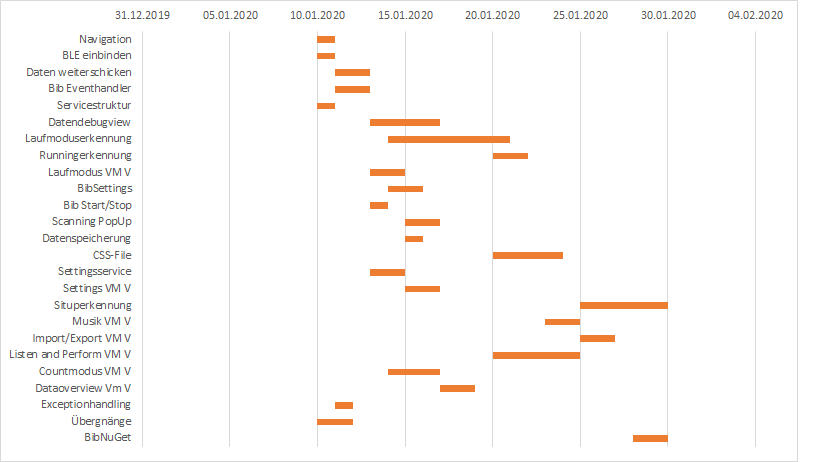
\includegraphics[width=\textwidth, height=0.5\textheight]{bilder/Implementierungsplan.png}

\subsection{Statistiken}
Mit der fortlaufenden Implementierung des Projektes haben sich einige interessante Daten gebildet, die nun präsentiert werden. Die wohl wichtigste Erfassung ist die Anzahl an Codezeilen (Lines of code (LOC)). Die Daten sind am 08.03.20 aufgenommen worden. Da das Projekt noch weiter entwickelt wird, handelt es sich nur um einen Zwischenstand der Daten.
\begin{itemize}
	\item \textit{Codezeilen (C\#): }15747
	\item \textit{Codezeilen (XML): }120
	\item \textit{Branches (max): }28
	\item \textit{Commits: }164
	\item \textit{Pullrequests: }40
	\item \textit{Tage: }35
	\item \textit{Gestellte Kriterien: }39
	\item \textit{Erfüllte Kriterien: }38
\end{itemize}
\section{Anhang}
\subsection{Links}
\subsubsection{Bibliothek}
NuGet Package: \url{https://www.nuget.org/packages/EarablesBLE}\\
GitHub Repository: \url{https://github.com/vlle1/lib-earablesKIT}
\subsubsection{App}
GitHub Repository: \url{https://github.com/vlle1/earablesKIT}
%%%%%%%%%%%%%%%%%%%%%%%%%%%%%%%%%%%%%%% END CONTENT %%%%%%%%%%%%%%%%%%%%%%%%%%%%%%%%%%%%%%%%%%%


\printglossaries
\stepcounter{section}


\end{document}